\documentclass[titlepage, 11pt, a4paper, ngerman]{article}
\usepackage[left=2cm, right=2cm, top=2cm, bottom=2cm]{geometry}
\usepackage[utf8]{inputenc}
\usepackage[acronym]{glossaries}
\usepackage[style=verbose]{biblatex}
\usepackage[nottoc]{tocbibind}
\usepackage{a4wide}
\usepackage{appendix}
\usepackage{babel}
\usepackage{amsmath}
\usepackage{tikz}
\usetikzlibrary{calc,patterns,angles,quotes}
\usepackage{graphicx}
\usepackage{titlepic}
\usepackage{wrapfig}
\usepackage{listings}
\usepackage{gensymb}
\usepackage{verbatim}
\usepackage{esvect}
\usepackage{hyperref}
\usepackage{xcolor}
\usepackage{qrcode}
\usepackage{minted}
\usepackage{csquotes}
\usepackage[bottom]{footmisc}

\usemintedstyle{vs}

\makeglossaries
\newglossaryentry{Tweak}{
    name=Tweak,
    description={Tweaks sind kleinere Anpassungen}
}
\newglossaryentry{Tool}{
    name=Tool,
    description={Als Tool (engl. \textit{tool}, 'Werkzeug', 'Hilfsmittel') wird ein Stück Software bezeichnet, welches eine bestimmte Funktion/Aufgabe übernimmt}
}
\newglossaryentry{Tracking}{
    name=Tracking,
    description={Tracking bezeichnet Verfolgung bzw. Überwachung}
}
\newglossaryentry{Assembler}{
    name=Assembler,
    description={Assembler-Code bezeichnet eine low-level Programmiersprache, die ein Computer ohne weitere Übersetzung verstehen und ausführen kann}
}
\newglossaryentry{Linker}{
    name=Linker,
    description={Als Linker (engl. \textit{to link}, 'verknüpfen', 'anschliessen') wird ein Tool bezeichnet, welches C/C++-Bibliotheken und C/C++-Quellcode zu einer ausführbaren Datei zusammenfügt}
}
\newglossaryentry{Compiler}{
    name=Compiler,
    description={Als Compiler wird ein programmiersprachspezifisches Tool bezeichnet, welches Quellcode in Assembler-Code übersetzen kann}
}
\newglossaryentry{Debugger}{
    name=Debugger,
    description={Als Debugger wird ein Tool bezeichnet, welches einem Programmierer hilft, Fehler (sog. engl. \textit{bugs}, 'Ungeziefer') in seinem Quellcode zu finden und zu beheben}
}
\newglossaryentry{Texteditor}{
    name=Texteditor,
    description={Als Texteditor wird ein Tool bezeichnet, mit welchem man Dateien bearbeiten kann}
}
\newglossaryentry{Linux}{
    name=Linux,
    description={Linux oder GNU/Linux bezeichnet eine Familie von Betriebssystemen für Computersysteme, basierend auf dem Linux-Kernel von Entwickler Linus Torvalds}
}
\newglossaryentry{Debian}{
    name=Debian,
    description={Debian bezeichnet eine Unterfamilie von Linux-Computersystemen. Dazu gehören z.B. Ubuntu, Linux Mint, Raspian etc...}
}
\newglossaryentry{Rendering}{
    name=Rendering,
    description={Als Rendering bezeichnet man ein Verfahren in der Computertechnik, bei welchem man durch Berechnungen audiovisuelle Ergebnisse produziert}
}
\newglossaryentry{Float}{
    name=Float,
    description={Ein Float oder eine Floating-Point-Zahl (engl. \textit{to float}, 'schweben', 'gleiten') ist ein Datentyp, welcher Kommazahlen bis zu einer gewissen Genauigkeit speichern kann (meist 32-bit). In der deutschen Sprache werden Floats gerne als Fliess- oder Gleitkommazahlen bezeichnet}
}
\newglossaryentry{Floating-Point}{
    name=Floating-Point,
    description={siehe \textbf{Float}}
}
\newglossaryentry{Makefile}{
    name=Makefile,
    description={Makefiles sind Kompilierungsinstruktionen, um ein grösseres Projekt richtig zu kompilieren}
}
\newglossaryentry{Engine}{
    name=Engine,
    description={Als eine Engine (engl. \textit{engine}, 'Motor', 'Antrieb') im programmiertechnischen Sinne wird ein Konstrukt verstanden, welches als Grundgerüst eines Programms angeschaut werden kann. Bei 3D-Videospielen und Applikationen zum Beispiel handelt es sich hierbei um den Programmteil, welcher 3D- zu 2D-Transformationen, Licht-/Schatten-/Farbberechnungen und physikalische Berechnungen wie Wurftrajektorien etc. vornimmt. Auf diesem Grundgerüst kann dann mit kleinsten Änderungen von höchstens einigen Zeilen Code ein neues Modell, eine neue Lichtquelle oder ein neues Geschoss in die Welt gesetzt werden und die Engine berechnet automatisch die neuen Umgebungs-/Bewegungsverhältnisse}
}
\newglossaryentry{Shader}{
    name=Shader,
    description={Als Shader wird ein kleines Programm bezeichnet, welches parallelisiert auf Grafikkarten ausgeführt wird. Es ist in GLSL geschrieben, einer zu C sehr ähnlichen Sprache. Shader werden in Grafik-API's über die Grafik-Pipeline angesteuert und dienen der parallelen Computation stets derselben Berechnungen}
}
\newglossaryentry{GitHub}{
    name=GitHub,
    description={GitHub (\url{https://github.com/}) ist eine Source-Code-Sharing-Plattform, basierend auf dem VCS \textit{Git}}
}
\newglossaryentry{Fragment}{
    name=Fragment,
    description={Als Fragments (engl. \textit{fragment}, 'Fragment', 'Bruchstück') werden Punkte auf einem Face eines Modells bezeichnet, welche durch die Rasterung des Faces in der Rasterization Stage entstehen. Die Framents werden in den Fragment Shadern eingefärbt}
}
\newglossaryentry{Vertex}{
    name=Vertex,
    description={Ein Vertex (engl. \textit{vertex}, 'Ecke', 'Eckpunkt', pl. \textit{vertices}) ist ein Punkt/Eckpunkt eines 3D-Modells. 3D-Modelle sind durch Vertices definiert und werden so respräsentiert}
}
\newglossaryentry{Vertices}{
    name=Vertices,
    description={siehe \textbf{Vertex}}
}
\newglossaryentry{Edge}{
    name=Edge,
    description={Als Edge (engl. \textit{edge}, 'Kante') werden Verbindungslinien zwischen zwei Vertices eines Modells bezeichnet}
}
\newglossaryentry{Face}{
    name=Face,
    description={Ein Face (engl. \textit{face}, 'Gesicht', 'Oberfläche', 'Fläche', pl. \textit{faces}) bezeichnet die Fläche, welche entsteht wenn die Vertices zu den primitiven Formen (Dreieck, Rechteck) zusammengefügt und durch Linien verbunden werden}
}
\newglossaryentry{Frame}{
    name=Frame,
    description={Ein Frame bezeichnet ein gerendertes Bild eines Programmes. Durch die Angabe der FPS lassen sich Aussagen über die Leistung von Applikationen machen}
}
\newglossaryentry{Frametime}{
    name=Frametime,
    description={Die Grösse der Frametime bezeichnet die Leistung einer Applikation, und wird meist in Millisekunden angegeben. Sie entspricht dem Kehrwert der FPS}
}
\newglossaryentry{Thread}{
    name=Thread,
    description={Als Thread (engl. \textit{thread}, 'Faden', 'Strang') wird eine parallele Ausführungskette in einem Computerprogramm beschrieben. Durch Threads kann ein Programm an mehreren Stellen gleichzeitig ausgeführt werden. Threads sind zentrale Objekte in der parallelisierten Programmierung}
}
\newglossaryentry{Multithreading}{
    name=Multithreading,
    description={Als Multithreading wird eine Programmiertechnik bezeichnet, wobei mehrere Threads benutzt werden um Software parallelisiert auszuführen}
}
\newglossaryentry{Fliesskommazahl}{
    name=Fliesskommazahl,
    description={siehe \textbf{Float}}
}
\newacronym{VCS}{VCS}{Version Control System}
\newacronym{IDE}{IDE}{Integrated Development Environment}
\newacronym{gcc}{gcc}{GNU Compiler Collection}
\newacronym{gdb}{gdb}{GNU Debugger}
\newacronym{CI}{CI}{Continuous Integration}
\newacronym{GUI}{GUI}{Graphical User Interface}
\newacronym{IFFT}{IFFT}{Inverse Fast Fourier Transform}
\newacronym{NaN}{NaN}{Not a Number}
\newacronym{LWJGL}{LWJGL}{Lightweight Java Game Library}
\newacronym{API}{API}{Application Programming Interface}
\newacronym{OpenGL}{OpenGL}{Open Graphics Library}
\newacronym{OpenGL ES}{OpenGL ES}{Open Graphics Library for Embedded Systems}
\newacronym{GLSL}{GLSL}{OpenGL Shading Language}
\newacronym{ASSIMP}{ASSIMP}{Open Asset Import Library}
\newacronym{GLFW}{GLFW}{Graphics Library Framework}
\newacronym{SDL}{SDL2}{Simple DirectMedia Layer 2.0}
\newacronym{GLM}{GLM}{OpenGL Mathematics}
\newacronym{FPS}{FPS}{Frames pro Sekunde}
\newacronym{CPU}{CPU}{Central Processing Unit}

\addbibresource{Literaturverzeichnis.bib}


\title{\large Maturitätsarbeit an der Kantonsschule Zürich Nord \\ \huge 3D-Rendering und Floating-Point: Vulkan und OpenGL als Grafik-API's im Vergleich}
\date{02. Dezember 2019}
\author{Cedric Schwyter \\ M6e \\ Betreut von: \\ Christian Prim}
\titlepic{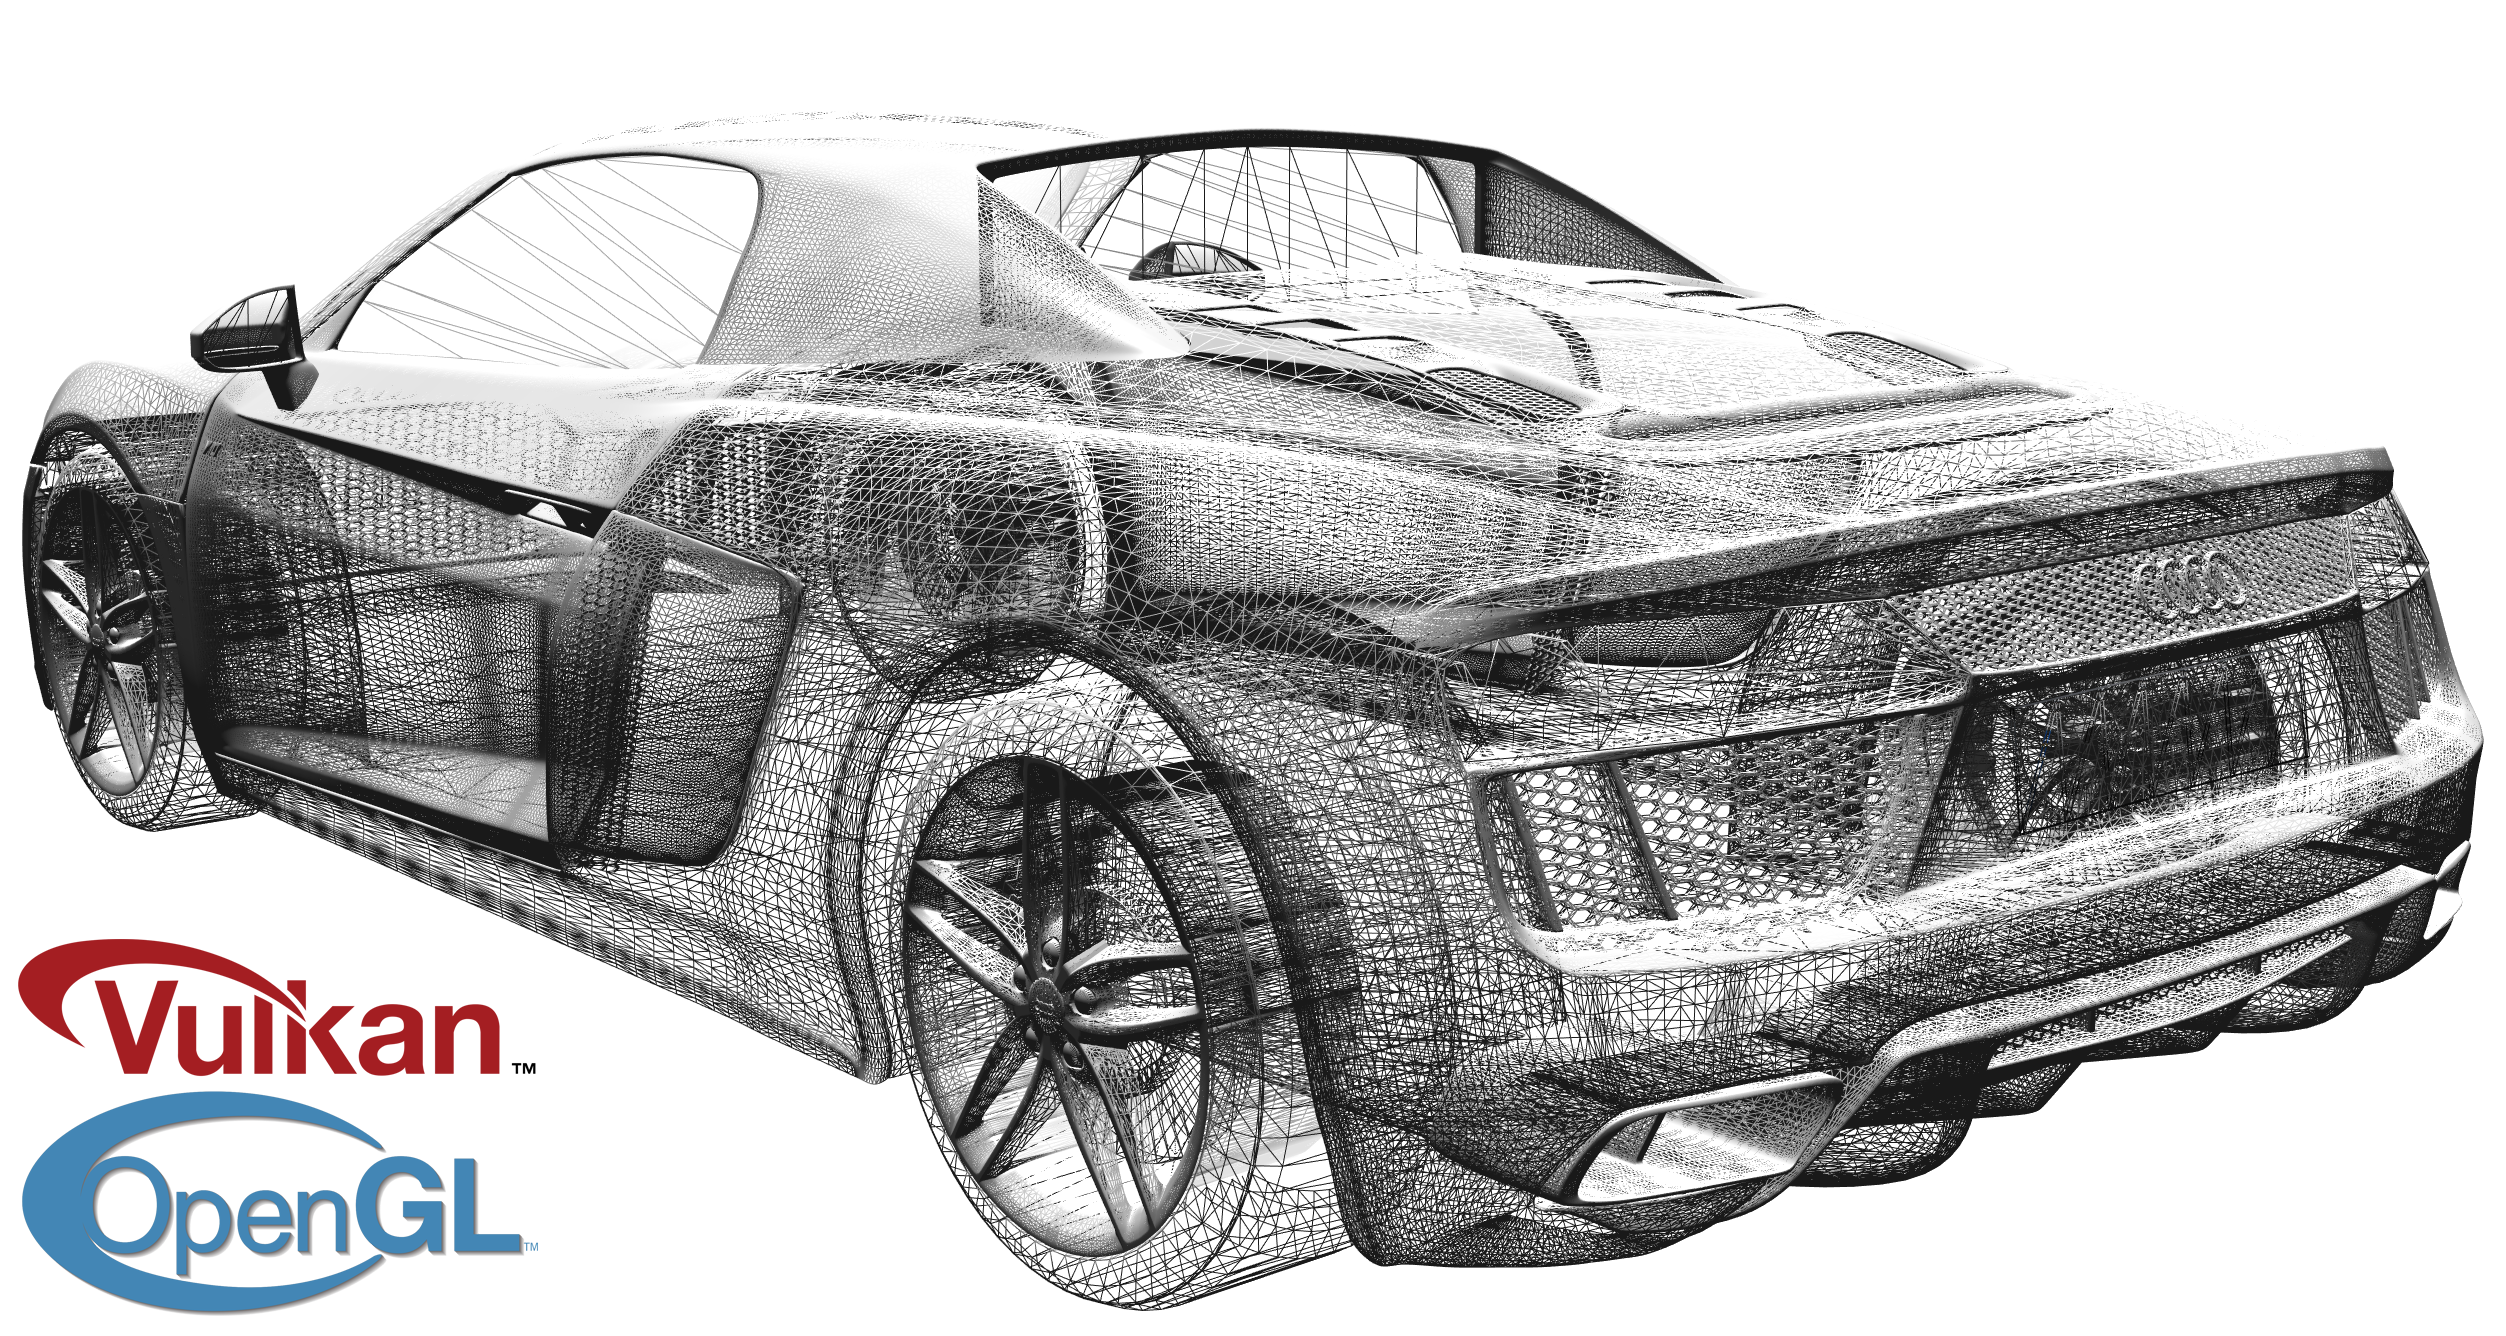
\includegraphics[width=\textwidth]{res/titlepic2.png}}

\begin{document}

\maketitle
\pagenumbering{gobble}


\newgeometry{left=2cm, right=2cm, top=2cm, bottom=2cm}
\newpage
\pagenumbering{Roman}
\tableofcontents

\newpage
\pagenumbering{arabic}
\section{Vorwort}
Da sich diese Arbeit auf einem ein wenig abstrakterem Niveau als dem typischen Anfänger-Program-mierlevel bewegt, wird minimales technisches und informatisches Grundverständnis vorausgesetzt, da es relativ unmöglich und völlig ausserhalb des Rahmens dieser Arbeit ist, die gesamten programmiertechnischen Basics zu erklären, welche hier angewendet werden. Die mathematische und physikalische Theorie zu den wichtigen Teilbereichen wird jedoch selbstverständlich erklärt, wobei auch hier ein basales mathematisches Verständnis und gewisse Grundkenntnisse vorausgesetzt werden, vor allem in der linearen Algebra, der Vektorgeometrie und der Analysis mit ihrer Differentialrechnung. \par
Weiterhin möchte ich an dieser Stelle meinen ausdrücklichen Dank an meinen lieben Kollegen Charpoan Kong, welcher mir ein wenig mit den \glspl{Makefile} und dem Port zu \gls{Linux} geholfen hat, und an meinen engagierten Betreuer Christian Prim, welcher meine Formeln stets zu korrigieren wusste, anbringen.\par
Dieses Thema wurde ausgewählt, da ich schon Vorwissen und Erfahrung in der Grafikprogrammierung hatte, wobei ich in \acrshort{OpenGL} heimischer war als in Vulkan. Ich habe bereits mehrere OpenGL-\glspl{Engine} in mehreren Programmiersprachen (C++, Java), jedoch erst eine einzige Vulkan-\gls{Engine} (C++) geschrieben. Ich persönlich sah es als Herausforderung für mich selbst, eine fähige \gls{Engine} mit Vulkan zu erstellen und ich glaube, dass ich diese auch gemeistert habe. Das Ganze wurde mit dem Hintergedanken der \gls{Floating-Point}-Ungenauigkeit angeschaut, welche oft ungewöhnliche Effekte nach sich zieht. Als Beispiel dafür gab es in diesem Projekt einen unbeabsichtigten Fall, bei welchem in einer Projektionsmatrix zwei \glspl{Float} von 8-byte- in 4-byte-Datentypen umgewandelt und erst nach dieser Umwandlung durcheinander geteilt wurden. Dadurch ging, vor allem bei kleinen Werten, sehr viel an Genauigkeit verloren. Dies führte zu irritierenden Verzerrungen der Projektion des dargestellten Raumes. Auf ein chaotisches System wie ein Doppelpendel angewandt entstehen durch \gls{Floating-Point}-Ungenauigkeiten sicherlich spannende Dinge. Dies war die Überlegung, welche sich stärker als erhofft bewahrheitet hat und auf Umwegen sogar dazu führte, dass ich mich sehr oberflächlich mit dem Lagrange-Formalismus auseinandergesetzt habe.\par
Das Titelbild wurde mit der Vulkan-Engine gerendert wobei mit internen Einstellungen der Polygon Mode verändert wurde, sodass das Modell nur als Netz aus Linien dargestellt wurde.


\newpage
\section{Einleitung}
Bei Vulkan und OpenGL handelt es sich um zwei High-Performance-Grafik-\acrshort{API}'s. Die beiden sollen in dieser Arbeit in der Theorie und vor allem in der Praxis verglichen werden. Über ein System des deterministischen Chaos sollen allfällige Unterschiede bezüglich der \gls{Floating-Point}-Ungenauigkeit der Endprodukte festgestellt werden.

\subsection{Konkrete Fragestellungen}
In dieser Arbeit wurde mit dem Fokus auf die folgenden Fragestellungen gearbeitet:
\begin{itemize}
    \item Ist \acrshort{OpenGL} immer noch eine geeignete Option im Jahr 2019?
    \item Was sind die Vor- und Nachteile von Vulkan gegenüber von \acrshort{OpenGL}? Ein theoretischer Vergleich.
    \item Programmierung von zwei Render-Engines mit der jeweiligen \acrshort{API} und einen Vergleich in der Praxis durchführen.
    \item Lässt sich ein Unterschied der beiden \glspl{Engine} bezüglich eines Systems des deterministischen Chaos (Doppelpendel) erkennen und wo könnten die Ursachen dafür liegen?
\end{itemize}


\subsection{Zielsetzungen}
Persönliche Zielsetzungen umfassten hierbei die korrekte und sinnvolle Programmierung der zwei Render-\glspl{Engine}. Die zwei Applikationen sollten vorzeigbare Resultate abliefern können und keine direkt erkennbaren Bugs und Fehler haben. Ausserdem sollten sie logisch, dynamisch und mit Möglichkei-ten der Weiterentwicklung programmiert werden, und nicht nur im Hinblick auf das deterministische Chaos. Dies war der persönliche Hauptfokus. Das System des deterministischen Chaos soll ausserdem physikalisch korrekt dargestellt werden.

\subsection{Vorgehen}
In einem ersten Teil wurden die zwei Render-\glspl{Engine} in C++17 programmiert. Dieser erste Teil umfasste circa 90\% der gesamten Arbeit. Insgesamt wurden rund 12'500 Zeilen Quellcode geschrieben, wobei jede einzelne von Hand getippt und alle Systeme selbst umgesetzt wurden. In einem zweiten Teil wurde dann das Doppelpendel-System in beiden Applikationen umgesetzt und auf mehreren Systemen getestet. Während der Entwicklung beider Programme wurde ein Arbeitsjournal geführt. Auf \gls{GitHub} sind die beiden Projekte mit Installationsanleitung zu finden (siehe Anhang A).

\subsection{Eigene Vorraussagen}
Da Vulkan viel neuer als OpenGL ist wurde angenommen, dass die Vulkan-Implementation performancetechnisch überlegen ist. Da noch nicht so viel Erfahrung mit Vulkan vorhanden war, wurde erwartet, dass Probleme mit der Implementation nicht immer auf dem besten Wege gelöst werden können. Dennoch wurde bei der Annahme, dass das Resultat von Vulkan besser als OpenGL's sein würde, geblieben. Grössere Schwierigkeiten bei der Entwicklung der Applikationen wurden nicht erwartet, da schon Erfahrung in der Grafikprogrammierung mit beiden \acrshort{API}'s vorhanden war. Für die Implementation des Doppelpendels wurde angenommen, dass dort physikalisch interessante Probleme auftreten könnten.


\newpage
\section{Grundlagen von 3D-Rendering}
Als \gls{Rendering} wird ein computertechnisches Verfahren bezeichnet, bei dem aufgrund von Berechnungen primär visuelle Ergebnisse produziert resp. Raum-Situationen simuliert werden. \gls{Rendering} als Begriff wird allerdings auch oft im Zusammenhang der Nachbearbeitung von Video-/Audiomaterial verwendet.\par Im Kontext von 3D-\gls{Rendering} spricht man von einer Simulation einer dreidimensionalen Welt/Umgebung mit Licht und allfälligen Schattenberechnungen, Farbberechnungen, Post Processing Effekten, Wellen-/Rauch-/Windsimulationen und vielem mehr. Zentral steht hierbei die Vektorgeometrie für Farb- und Lichtberechnungen, sowie die Matrizenrechnung mit ihren Transformationsmatrizen.

\subsection{Was ist eine Grafik-API?}
Als \acrfull{API} wird im Allgemeinen eine Programmierschnittstelle bezeichnet, welche das Ansteuern von Software oder Hardware direkt aus dem Quellcode erlaubt. Diese Soft- oder Hardware kann sich auf demselben Computersystem, aber auch auf einem Servercluster am anderen Ende der Welt befinden. Die Schnittstelle vereinfacht vor allem das Benutzen von externen, aber auch systeminternen Computations- und Informationsbeschaffungsmöglichkeiten. Viele Technikunternehmen stellen deswegen auch eine eigene \acrshort{API} bereit, um Programmierern die Integration der angebotenen Dienste zu vereinfachen.\footcite{apis} Bekannte Beispiele dafür wären die Google Maps \acrshort{API}, die YouTube \acrshort{API} oder die NASA \acrshort{API}.\par
Im Sinne der Grafikprogrammierung wird unter einer Grafik-\acrshort{API} eine Vereinfachung der Ansteuerung von Computing-Potenzial auf Grafikkarten verstanden. Grafikkarten sind auf hochgradig parallelisierte Computation ausgelegte High-Performance-Prozessorchips. Parallelisierung meint dabei die simultane Durchführung der ein- und derselben Berechnungen auf einigen hundert bis zu mehreren tausend Rechenkernen für übliche Endbenutzer-Grafikkarten.\footcite{cuda-cores} Dadurch, dass die Berechnungen gleichzeitig tausendfach durchgeführt werden können, müssen sie nicht nacheinander ausgeführt werden und sparen somit viel wertvolle Zeit.

\subsection{Repräsentation von 3D-Modellen}
3D-Modelle werden typischerweise als eine Reihe von Punkten (die \textit{\gls{Vertices}}), welche durch Linien (die \textit{\glspl{Edge}}) miteinander verbunden werden und somit Flächen (die \textit{\glspl{Face}}) bilden, repräsentiert. Die Faces werden weiter in \textit{\glspl{Fragment}} gerastert. Diese entsprechen einfärbbaren Punkten auf dem Face. Die Farbe des jeweiligen \gls{Fragment}s wird im \gls{Fragment} \gls{Shader} berechnet. Den Zusammenhang \gls{Vertex}, \gls{Edge} und \gls{Face} kann man sich wörtlich übersetzt als Ecke, Kante und Fläche vorstellen. Auf dem Titelbild sind die Edges eines Modells, welches aus 1'036'416 Vertices besteht, dargestellt. Je nach Geometrie des Modells wird dieses zu Dreiecken, Vierecken oder anderen Polygonen verbunden. Je nach Modell kann die Wahl der Geometrie eine Rolle spielen, da z.B. Würfel nicht unbedingt aus Dreiecken geformt werden müssen, sondern Vierecke ausreichen. Somit hätte man weniger Faces (nämlich nur 6 anstatt 12), was Rechenaufwand einsparen würde. Am weitesten verbreitet sind jedoch trotzdem Dreiecke, da sich grössere Polygone immer aus mehreren kleineren Dreiecken formen lassen. Die dreieckigen \glspl{Face} können dann eingefärbt und texturiert werden. In einer Modelldatei befinden sich also eine Reihe von 3D-Punkten und zusätzliche Informationen. Weiter können zum Beispiel Texturkoordinaten, Normalenvektoren der \glspl{Face}, Farben, Tangenten/Bitangenten oder sonstige Zusatzdaten in den Modelldateien abgelegt werden. Texturkoordinaten bestimmen, welcher Teil einer Textur auf welchen Teil des \glspl{Face} gemappt (also projiziert) wird. Die Normalenvektoren zum Beispiel werden für die später erklärten Lichtberechnungen benötigt. Der Rest war für die Applikationen irrelevant. Die beiden \glspl{Engine} wurden mithilfe der Model-Loading-Library \acrshort{ASSIMP} geschrieben, welche verschiedenste 3D-Modellformate laden und parsen kann, wobei das wichtigste und verbreitetste davon das \textit{.obj}-Format ist.

\subsection{Mathematische Grundlagen}
Vorkenntnisse in der linearen Algebra und der Vektorrechnung werden vorausgesetzt um die folgenden Sachverhalte zu verstehen.\par
Die erste Schwierigkeit, die beim Rendern von 3D-Räumen auftaucht, ist die Darstellung auf einem 2D-Bildschirm. Irgendwie müssen dreidimensionale Raumkoordinaten auf zweidimensionale Bildschirmkoordinaten projiziert werden. Dies stellt sich als fundamentale Frage, denn, wenn dies nicht geklärt werden kann, können zwangsweise keine visuellen Ergebnisse entstehen. Die Werkzeuge, um dieses Problem zu lösen bietet die Matrizenrechnung mit Transformationsmatrizen. In der Grafikprogrammierung werden nach Konvention 4-dimensionale Vektoren folgender Form verwendet, wobei $w$ standardmässig auf 1 gesetzt wird, sofern keine spezielle Verwendung für diese vierte Komponente besteht: 
\begin{align*}
    \begin{pmatrix}
    x \\
    y \\
    z \\
    w
    \end{pmatrix} 
\end{align*}
\bigbreak
Das heisst, alle dreidimensionalen Vektoren in der Grafikrechnung können ebenfalls als vierdimensionale Vektoren, deren vierte Komponente 1 ist, dargestellt werden. Zum Beispiel werden Farbwerte mit 3 Kanälen (RGB) durch so einen Vektor mit $w = 1$, und Farbwerte mit 4 Kanälen (RGBA) als normalen vierdimensionalen Vektor (bei welchem $w$ dem Wert des vierten Kanals entspricht) repräsentiert. Dieser Konvention und den mathematischen Rechengesetzen zufolge werden auch $4\times4$-Matrizen verwendet da die Matrixmultiplikation mit einem Vektor sonst nicht definiert wäre. Zunächst werden die benötigten Transformationen für die nachfolgenden theoretischen Betrachtungen erläutert.\footcite{transformations}


\subsubsection{Skalierung}
Ein Vektor kann mit einer Matrix wie folgt um den Skalierungsvektor $\begin{pmatrix}
    a \\
    b \\
    c
    \end{pmatrix}$ skaliert werden:
\begin{align*}
    \begin{bmatrix} 
    a & 0 & 0 & 0 \\
    0 & b & 0 & 0 \\
    0 & 0 & c & 0 \\
    0 & 0 & 0 & 1
    \end{bmatrix} \cdot
    \begin{pmatrix}
    x \\ y \\ z \\ 1
    \end{pmatrix} &= 
    \begin{pmatrix}
    a \cdot x \\
    b \cdot y \\
    c \cdot z \\
    1
    \end{pmatrix}
\end{align*}

\subsubsection{Translation}
Eine Translation um den Verschiebungsvektor $\begin{pmatrix}
    a \\
    b \\
    c
    \end{pmatrix}$ sieht folgendermassen aus:
\begin{align*}
    \begin{bmatrix} 
    1 & 0 & 0 & a \\
    0 & 1 & 0 & b \\
    0 & 0 & 1 & c \\
    0 & 0 & 0 & 1
    \end{bmatrix} \cdot
    \begin{pmatrix}
    x \\ y \\ z \\ 1
    \end{pmatrix} &= 
    \begin{pmatrix}
    a + x \\
    b + y \\
    c + z \\
    1
    \end{pmatrix}
\end{align*}
\bigbreak
Die Translation bezeichnet grundsätzlich die Addition zweier Vektoren. Aus diesem Zusammenhang folgt sogleich, dass sich jeder 3D-Vektor auch als eine $4\times4$-Matrix ausdrücken lässt. Dies lässt sich ganz einfach darstellen wenn $x$, $y$ und $z = 0$ sind:
\begin{align*}
    \begin{bmatrix}
    1 & 0 & 0 & a \\
    0 & 1 & 0 & b \\
    0 & 0 & 1 & c \\
    0 & 0 & 0 & 1
    \end{bmatrix} \cdot
    \begin{pmatrix}
    0 \\ 0 \\ 0 \\ 1
    \end{pmatrix} &=
    \begin{pmatrix}
    a + 0 \\
    b + 0 \\
    c + 0 \\
    1
    \end{pmatrix} = 
    \begin{pmatrix}
    a \\
    b \\
    c \\
    1
    \end{pmatrix} \widehat{=}
    \begin{pmatrix}
    a \\
    b \\
    c
    \end{pmatrix}
\end{align*}
\bigbreak
Später wird dann teilweise nur noch mit 3-Komponenten-Vektoren gerechnet, welche einfach als 4-Komponenten-Vektoren mit vierter Komponente $w = 1$ angeschaut werden können. Das wird in der Grafikprogrammierung zur Vereinfachung manchmal gemacht.

\subsubsection{Rotation}
Ein Vektor kann um eine (beliebige) Achse gedreht werden. Durch eine Transformationsmatrix ausgedrückt, sehen Rotationen wie folgt aus: \bigbreak
Um die x-Achse $
\begin{pmatrix}
1 \\
0 \\
0 \\
1
\end{pmatrix}$ mit Winkel $\theta$:
\begin{align*}
    \begin{bmatrix} 
    1 & 0 & 0 & 0 \\
    0 & \cos{\theta} & - \sin{\theta} & 0 \\
    0 & \sin{\theta} & \cos{\theta} & 0 \\
    0 & 0 & 0 & 1
    \end{bmatrix} \cdot
    \begin{pmatrix}
    x \\ y \\ z \\ 1
    \end{pmatrix} &= 
    \begin{pmatrix}
    x \\
    \cos{\theta} \cdot y - \sin{\theta} \cdot z \\
    \sin{\theta} \cdot y + \cos{\theta} \cdot z \\
    1
    \end{pmatrix}
\end{align*}
\bigbreak
Um die y-Achse $
\begin{pmatrix}
0 \\
1 \\
0 \\
1
\end{pmatrix}$ mit Winkel $\theta$:
\begin{align*}
    \begin{bmatrix} 
    \cos{\theta} & 0 & \sin{\theta} & 0 \\
    0 & 1 & 0 & 0 \\
    - \sin{\theta} & 0 & \cos{\theta} & 0 \\
    0 & 0 & 0 & 1
    \end{bmatrix} \cdot
    \begin{pmatrix}
    x \\ y \\ z \\ 1
    \end{pmatrix} &= 
    \begin{pmatrix}
    \cos{\theta} \cdot x + \sin{\theta} \cdot z \\
    y \\
    - \sin{\theta} \cdot x + \cos{\theta} \cdot z \\
    1
    \end{pmatrix}
\end{align*}
\bigbreak
Um die z-Achse $
\begin{pmatrix}
0 \\
0 \\
1 \\
1
\end{pmatrix}$ mit Winkel $\theta$:
\begin{align*}
    \begin{bmatrix} 
    \cos{\theta} & - \sin{\theta} & 0 & 0 \\
    \sin{\theta} & \cos{\theta} & 0 & 0 \\
    0 & 0 & 1 & 0 \\
    0 & 0 & 0 & 1
    \end{bmatrix} \cdot
    \begin{pmatrix}
    x \\ y \\ z \\ 1
    \end{pmatrix} &= 
    \begin{pmatrix}
    \cos{\theta} \cdot x - \sin{\theta} \cdot y \\
    \sin{\theta} \cdot x + \cos{\theta} \cdot y \\
    z \\
    1
    \end{pmatrix}
\end{align*}
\bigbreak
Um eine beliebige Achse $
\begin{pmatrix}
a \\
b \\
c \\
1
\end{pmatrix} $ für die gilt $ \Biggl|\begin{pmatrix}
a \\
b \\
c
\end{pmatrix}\Biggl| = 1$ mit Winkel $\theta$:
\begin{align*}
    \begin{bmatrix} 
    \cos{\theta} + a^{2} \cdot (1 - \cos{\theta}) & a \cdot b \cdot (1 - \cos{\theta}) - c \cdot \sin{\theta} & a \cdot c \cdot (1 - \cos{\theta}) + b \cdot \sin{\theta} & 0 \\
    b \cdot a \cdot (1 - \cos{\theta}) + c \cdot \sin{\theta} & \cos{\theta} + b^{2} \cdot (1 - \cos{\theta}) & b \cdot c \cdot (1 - \cos{\theta}) - a \cdot \sin{\theta} & 0 \\
    c \cdot a \cdot (1 - \cos{\theta}) - b \cdot \sin{\theta} & c \cdot b \cdot (1 - \cos{\theta}) + a \cdot \sin{\theta} & \cos{\theta} + c^{2} \cdot (1 - \cos{\theta}) & 0 \\
    0 & 0 & 0 & 1
    \end{bmatrix} \cdot
    \begin{pmatrix}
    x \\ y \\ z \\ 1
    \end{pmatrix} \\ =
    \begin{pmatrix}
    x \cdot (\cos{\theta} + a^{2} \cdot (1 - \cos{\theta})) + y \cdot (a \cdot b \cdot (1 - \cos{\theta}) - c \cdot \sin{\theta}) + z \cdot (a \cdot c \cdot (1 - \cos{\theta}) + b \cdot \sin{\theta}) \\
    x \cdot (b \cdot a \cdot (1 - \cos{\theta}) + c \cdot \sin{\theta}) + y \cdot (\cos{\theta} + b^{2} \cdot (1 - \cos{\theta})) + z \cdot (b \cdot c \cdot (1 - \cos{\theta}) - a \cdot \sin{\theta}) \\
    x \cdot (c \cdot a \cdot (1 - \cos{\theta}) - b \cdot \sin{\theta}) + y \cdot (c \cdot b \cdot (1 - \cos{\theta}) + a \cdot \sin{\theta}) + z \cdot (\cos{\theta} + c^{2} \cdot (1 - \cos{\theta})) \\
    1
    \end{pmatrix}
\end{align*} 
\bigbreak
Diese Transformationsmatrizen werden sehr schnell sehr mühsam. Um dies anschaulich darzustellen wurde die Rotationsmatrix für eine Drehung um eine beliebige Achse abgebildet. Deswegen wird die lineare Algebra in beiden Applikationen von einer Bibliothek namens \acrfull{GLM} übernommen, damit keine eigene Lösung implementiert werden muss.\par
Durch Matrizen lassen sich Vektoren also manipulieren und transformieren, wie man will. Durch die Matrizenmultiplikation können mehrere Transformationen miteinander verknüpft und in einer einzigen Matrix dargestellt werden. Durch diese Möglichkeiten der Veränderung von Vektoren kann die nachfolgend erklärte Übersetzung von 3D zu 2D durchgeführt werden. Zuerst jedoch müssen Koordinatensysteme eingeführt werden, welche oft benötigt werden.

\subsection{Koordinatensysteme}
In der Grafikprogrammierung trifft man verschiedene Koordinatensysteme an, welche allesamt für gewisse Operationen benötigt werden. Sie werden allesamt auf Englisch bezeichnet. Die $MVP$-Matrizen, welche in der Folge erklärt sind, werden auch auf Englisch bezeichnet. Es werden also die folgenden Koordinatensysteme benötigt:
\begin{itemize}
    \item Local Space
    \item World Space
    \item View Space
    \item Clip Space
    \item Screen Space
\end{itemize}
Sie verhalten sich zueinander wie Abbildung \ref{fig:coordinate-systems} zeigt und werden im nächsten Unterkapitel anhand der tatsächlichen Anwendung erklärt.
\begin{figure}[ht]
    \centering
    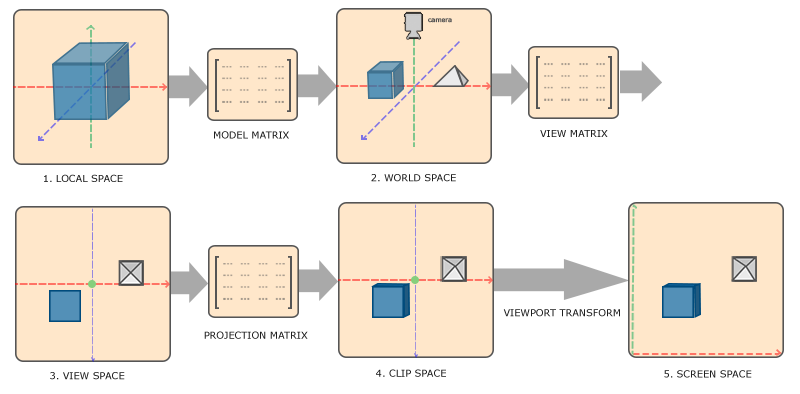
\includegraphics[scale=0.55]{res/coordinate_systems.png}
    \caption[Koordinatensysteme und $MVP$-Transform]{Koordinatensysteme und $MVP$-Transform\footnotemark}
    \label{fig:coordinate-systems}
\end{figure}
\footcitetext{coordinate-systems}

\subsection{Anwendung für 3D- zu 2D-Transformation}
Wie kann dieses Vorwissen nun dazu dienen, 3D-Raumkoordinaten in 2D-Bildschirmkoordinaten umzurechnen? Angenommen, man hat ein 3D-Modell welches man rendern möchte. Dazu müssen nun die 3D-\gls{Vertices} in 2D-Punkte transformiert werden. Dies läuft nach folgendem Schema ab: Die \gls{Vertices} des Modells sind relativ zu seinem Ursprung, der meist innerhalb des Modells selbst liegt, angegeben. Dies nennt sich Local Space. Diese Koordinaten werden mithilfe der Model-Matrix ($M$) in World Space-Koordinaten umgewandelt. Die Model-Matrix bestimmt wo ($\widehat{=}$ Translation), mit welcher Grösse ($\widehat{=}$ Skalierung) und mit welcher Ausrichtung ($\widehat{=}$ Rotation) das Modell schlussendlich im Raum landet. Die View-Matrix ($V$) rechnet diese World Space-Koordinaten in ihre View Space-Äquivalente um. View Space bezeichnet die Koordinaten aus der Sicht der Kamera, ohne jegliche perspektivische oder orthographische Projektionen. Die perspektivische oder orthographische Projektion übernimmt die Projection Matrix ($P$); sie verwandelt die View Space-Koordinaten in Clip Space-Koordinaten. 'Clip Space', weil die Kamera nur einen gewissen Ausschnitt des gesamten Raumes zeigen kann, welcher im sogenannten \textit{View Frustum} liegt, der Rest wird 'geclipped' (= weggeschnitten). Dies nennt sich auch Model-View-Projection-Transform (oder kurz $MVP$-Transform). Durch den Viewport Transform, welcher die Auflösung der Ausgabe und den festgelegten Ausschnitt durch den Benutzer bestimmt, werden Clip Space dann schlussendlich zu Screen Space-Koordinaten, den finalen Bildschirmkoordinaten. Diese geben an, auf welchem Pixel des Displays ein Vertex zu liegen kommen muss, um eine realistische Darstellung des 3D-Raumes zu erhalten. In Abbildung \ref{fig:coordinate-systems} ist dies anschaulich dargestellt.\par
Durch die Nicht-Kommutativität der Matrixmultiplikation müssen die Matrizen in der richtigen Reihenfolge miteinander multipliziert werden. Diese wäre aufgrund der Definition der Matrizenmultiplikation sogesehen 'rückwärts':
\begin{align*}
    T_{\text{res}} &= P \cdot V \cdot M
\end{align*}
\bigbreak
Diese Gleichung konstituiert die fundamentalen Prinzipien der Grafikprogrammierung. Mit ihr lässt sich die resultierende Transformationsmatrix $T_{\text{res}}$ berechnen. Angewandt auf die tatsächlichen Positions-/Ortsvektoren $\vec{OV}$ der \gls{Vertices}, wie sie in der 3D-Modelldatei abgespeichert sind, entspricht dies:
\begin{align*}
    \vec{P}_{\text{res}} &= T_{\text{res}} \cdot \vec{OV} = P \cdot V \cdot M \cdot \vec{OV}
\end{align*}
\bigbreak
$\vec{P}_{\text{res}}$ entspricht dabei den resultierenden Screen Space-Koordinaten. Auch hier handelt es sich um einen 4-dimensionalen Vektor, von welchem jedoch prinzipiell nur die ersten zwei Komponenten benötigt werden. Der Rest wird deswegen wie gewohnt ignoriert. \par
Diese Matrizenmultiplikation findet in den \gls{Vertex} \gls{Shader}n statt. Standard-\gls{Vertex}-\gls{Shader}, wie sie bei den beiden Programmen tatsächlich eingesetzt werden, können im Anhang C eingesehen werden.

\subsection{Kamera}
\acrshort{OpenGL} und Vulkan kennen beide das Prinzip einer Kamera nicht. Der Programmierer muss sich also selbst eine Lösung überlegen. Da das Prinzip einer Kamera für die Grafik-\acrshort{API}'s unbekannt ist, wird der 3D-Raum invers den Inputs des Benutzers bewegt. Wenn der Benutzer sich nach links bewegen möchte, bewegt sich nicht die Kamera nach links, sondern die Welt nach rechts. Wenn der Benutzer nach oben schauen will, rotiert nicht die Kamera nach oben, sondern die Welt nach unten. Und hier kommt die View-Matrix ins Spiel. Die Model-Matrix bestimmt Position, Ausrichtung und Grösse des Modells und die Projection-Matrix sorgt für perspektivische Verzerrungen. Noch macht die View-Matrix nichts von Belang. Analog zur Model-Matrix könnte die View-Matrix die Position und Ausrichtung nicht des Objektes, sondern des gesamten Raumes relativ zur vom Programmierer eingeführten Kamera bestimmen. Und das wird in der Praxis auch so gemacht. Der Positionsvektor der Kamera wird als $\vec{P}$ bezeichnet. Das View Space-Koordinatensystem hat seinen Ursprung in der Kamera und ist durch drei senkrecht stehende Vektoren, den Up-Vektor $\vec{U}$, den Right-Vektor $\vec{R}$ und den Direction-Vektor $\vec{D}$, definiert. Abbildung \ref{fig:view-space} veranschaulicht dies.
\begin{figure}[ht]
    \centering
    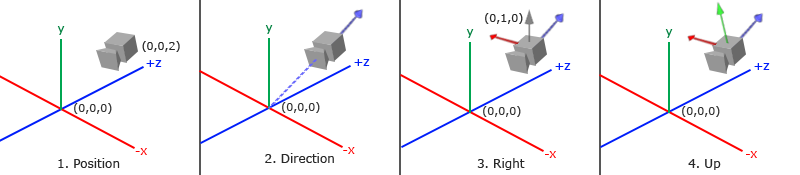
\includegraphics[scale=0.4]{res/camera_axes.png}
    \caption[View Space-Koordinatensystem]{View Space-Koordinatensystem\footnotemark}
    \label{fig:view-space}
\end{figure}
\footcitetext{logl-camera}
Der Direction-Vektor $\vec{D}$ zeigt hierbei hinten aus der Kamera hinaus. Dies ist jedoch Definitionssache, da ein einziges Vorzeichen den Unterschied macht. Alle Vektoren bis auf $\vec{P}$ sind normiert. Die folgende Matrix wird gemeinhin als LookAt-Matrix bezeichnet. Dabei geht es darum, eine Transformationsmatrix zu finden, wenn die Positon und das Target $\vec{T}$ der Kamera, also wo die Kamera hinblickt, gegeben ist.\footcite{camera} Weiterhin gibt es noch den World Up-Vektor (bei Vulkan mit negativem Vorzeichen, da dort die $y$-Achse in die andere Richtung zeigt): 
\begin{align*}
    \vec{WU} = \begin{pmatrix}
    0 \\
    1 \\
    0
    \end{pmatrix}
\end{align*}
\bigbreak
Die $\vec{U}$, $\vec{R}$ und $\vec{D}$ Vektoren lassen sich zu jedem Zeitpunkt relativ einfach berechnen:
\begin{align*}
    \vec{D} &= \frac{\vec{P} - \vec{T}}{|\vec{P} - \vec{T}|} \\
    \vec{R} &= \frac{\vec{WU} \times \vec{D}}{|\vec{WU} \times \vec{D}|} \\
    \vec{U} &= \vec{D} \times \vec{R}
\end{align*}
\bigbreak
$\vec{U}$ muss nicht normiert werden, da er aus dem Kreuzprodukt zweier bereits normierter Vektoren berechnet wird. Wenn ein Koordinatensystem wie das View Space-System durch 3 senkrechte Achsen definiert ist, lässt sich eine Matrix, welche Vektoren in dieses Koordinatensystem transformiert, erstellen.\par
In diesem Zusammenhang wird die Übersetzung von World Space- in View Space-Koordinaten vorgenommen, wobei exakt diese Transformation auf eine vorhergehende Verschiebung um die Position der Kamera angewendet wird. Diese Matrix wird dann LookAt-Matrix genannt\footcite{camera}:
\begin{align*}
    \text{LookAt} &= 
    \begin{bmatrix}
    R_{x} & R_{y} & R_{z} & 0 \\
    U_{x} & U_{y} & U_{z} & 0 \\
    D_{x} & D_{y} & D_{z} & 0 \\
    0 & 0 & 0 & 1
    \end{bmatrix} \cdot 
    \begin{bmatrix}
    1 & 0 & 0 & -P_{x} \\
    0 & 1 & 0 & -P_{y} \\
    0 & 0 & 1 & -P_{z} \\
    0 & 0 & 0 & 1
    \end{bmatrix} \\ &=
    \begin{bmatrix}
    R_{x} & R_{y} & R_{z} & -P_{x} \cdot R_{x} - P_{y} \cdot R_{y} - P_{z} \cdot R_{z} \\
    U_{x} & U_{y} & U_{z} & -P_{x} \cdot U_{x} - P_{y} \cdot U_{y} - P_{z} \cdot U_{z} \\
    D_{x} & D_{y} & D_{z} & -P_{x} \cdot D_{x} - P_{y} \cdot D_{y} - P_{z} \cdot D_{z} \\
    0 & 0 & 0 & 1
    \end{bmatrix}
\end{align*}
\bigbreak
Diese LookAt-Matrix beinhaltet nun also die genaue Position ($\vec{P}$) und Ausrichtung ($\vec{R}$, $\vec{U}$ und $\vec{D}$) der Kamera. Genau die Bedingungen, die für die View-Matrix gelten. Somit ist die View-Matrix definiert und sorgt dafür, dass der Benutzer seine virtuelle Kamera bewegen und rotieren kann. In tatsächlichen Applikationen wird mit den sogenannten Eulerschen Winkeln gearbeitet. 
\begin{figure}[ht]
    \centering
    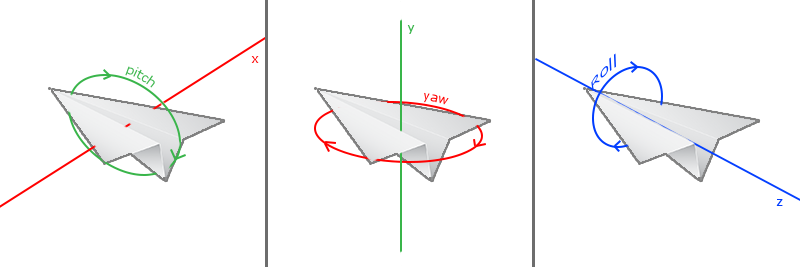
\includegraphics[scale=0.4]{res/euler-angles2.png}
    \caption[Eulersche Winkel anhand eines Flugzeugs]{Eulersche Winkel anhand eines Flugzeugs\footnotemark}
    \label{fig:euler-angles}
\end{figure}
\footcitetext{logl-camera}
Diese bezeichnen die Rotation um jede der drei Achsen im Raum. In unserem Fall liegen die Bezeichnungen wie in Abbildung \ref{fig:euler-angles}: Der Pitch $\theta$ für die $x$-Achse, Yaw $\psi$ für die $y$-Achse und Roll $\phi$ für die $z$-Achse. Die Mausbewegungen des Users können als solche Winkel interpretiert werden. Durch einfache Trigonometrie kann dann der $\vec{D}$-Vektor berechnet werden:
\begin{align*}
    \vec{D} &= \begin{pmatrix}
    \cos{\theta} \cdot \cos{\psi} \\
    \sin{\theta} \\
    \cos{\theta} \cdot \sin{\psi}
    \end{pmatrix}
\end{align*}
\bigbreak
Da der Roll $\phi$ meistens nur bei Flugsimulatoren gebraucht wird, sieht dieser Vektor $\vec{D}$ in vielen Programmen so aus. Durch diese relativ einfachen Zusammenhänge funktioniert die vom Programmierer eingeführte Kamera in einem Videospiel oder einer 3D-Simulation.

\subsection{Phong-Lighting}
Ein wichtiger Bestandteil einer jeden Grafikapplikation, welche auf eine realitätsnahe Darstellung des Raumes abzielt, sind annähernd gute Berechnungen der Lichtverhältnisse. Ein Modell, welches sich durchgesetzt und bewährt hat, ist das sogenannte \textit{Phong-Lighting} oder dessen Weiterentwicklung \textit{Blinn-Phong-Lighting}. Dieses versucht, die geometrische Optik der Farbempfindung nachzuahmen. Dabei werden verschiedene Komponenten des Lichts unterschieden. \footcite{logl-lighting}

\subsubsection{Ambient Lighting} 
Es gibt das \textit{Ambient Lighting}, welches als Umgebungslicht verstanden werden kann. Dies setzt sich in der echten Welt aus reflektiertem Licht von allen möglichen Oberflächen zusammen. Da dies rechentechnisch sehr schwer zu simulieren ist, wird normalerweise einfach eine bestimmte Menge an Umgebungsbeleuchtung angenommen. 

\subsubsection{Diffuse Lighting}
Weiter existiert das \textit{Diffuse Lighting}. Dies dient der Berechnung der direkten Beleuchtung eines \glspl{Face} durch eine Lichtquelle mithilfe von ein paar vektorgeometrischen Eigenschaften. Über das Skalarprodukt des Vektors, welcher zur Lichtquelle zeigt, mit dem Normalenvektor des \glspl{Face} kann ein Koeffizient für die Erhellung berechnet werden. Abbildung \ref{fig:diffuse} zeigt dies schematisch.
\begin{figure}[ht]
    \centering
    
\includegraphics[scale=0.35]{res/diffuse_light.png}
    \caption[Diffuse Lighting im Querschnitt des \glspl{Face}]{Diffuse Lighting im Querschnitt des \glspl{Face}\footnotemark}
    \label{fig:diffuse}
\end{figure}
\footcitetext{logl-lighting}

\subsubsection{Specular Lighting}
Zu guter Letzt kommt das \textit{Specular Lighting}. Es dient der Simulation von reflektionsbedingten optischen \textit{Highlights}. Dies kann anschaulich an folgendem Beispiel erklärt werden: Man stelle sich ein Auto vor, welches durch die Metallkarosserie eine grosse optische Reflektivität hat. Die Sonne wird reflektiert, an gewissen Stellen stärker als an anderen, sodass man sogar geblendet wird. Um diese direkte Reflektion zu simulieren, wird auch hier über das Skalarprodukt des am Normalenvektor des \glspl{Face} reflektierten Vektors mit dem Vektor, der zur Quelle zeigt, ein Koeffizient zur weiteren Aufhellung berechnet. Abbildung \ref{fig:specular} stellt dies auch hier schematisch dar.
\begin{figure}[ht]
    \centering
    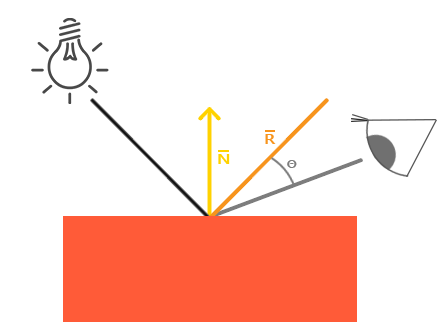
\includegraphics[scale=0.35]{res/specular_light.png}
    \caption[Specular Lighting im Querschnitt des \glspl{Face}]{Specular Lighting im Querschnitt des \glspl{Face}\footnotemark}
    \label{fig:specular}
\end{figure}
\footcitetext{logl-lighting}

Die Kombination dieser drei Elemente zusammen ergibt eine relativ gute Simulation der Lichtverhältnisse, welche nicht zu viel Rechenaufwand abverlangt. In Anhang C können die jeweiligen Implementationen in den \gls{Fragment} \gls{Shader}n für beide Applikationen eingesehen werden. Früher, als Grafikkarten noch nicht so leistungsfähig waren wie heute, wurden diese Berechnungen nicht pro \gls{Fragment}, sondern pro \gls{Vertex} in den \gls{Vertex} \gls{Shader}n durchgeführt. Dies führte zu massiven Leistungsverbesserungen, aber auch zu einer Verfälschung des Resultats. Dies wurde dann Gouroud-Lighting genannt.\footcite{logl-lighting}

\subsection{Probleme und Schwierigkeiten}
Diese vorhin erwähnten Rotationsmatrizen führen ein Problem, das unter dem Namen \textit{Gimbal Lock} bekannt ist, ein. Dies entsteht vor allem dann, wenn anstatt um eine einzige Achse, um mehrere Achsen rotiert wird. Beispielsweise wird zuerst um die $x$-Achse, dann um die $y$-Achse rotiert, anstatt direkt um eine Achse, die dazwischen liegt. Die Rotationsmatrix um eine beliebige Achse schwächt diese Gimbal Lock ein wenig ab, kann sie jedoch nicht vollständig verhindern.\footcite{transformations} Bei der Gimbal Lock entsteht eine exakte Überlagerung zweier Achsen, wonach nur noch um zwei anstatt um drei Achsen rotiert werden kann. Um dies zu verhindern wurde im tatsächlichen Quellcode dann eine Begrenzung der Rotationswinkel der Kamera eingebaut, damit exakt dieses Problem nicht auftritt. Gimbal Lock tritt dann auf, wenn ein Rotationswinkel $\pm 90.0\degree$ erreicht. Das heisst, es muss sichergestellt sein, dass keiner der drei Rotationswinkel der Kamera jemals einen Wert von $\pm 90.0\degree$ annimmt. Da die Kamera in den Applikationen sich jedoch nur in zwei Richtungen steuern lässt (oben/unten, links/rechts) muss nur garantiert werden, dass der Pitch-Winkel niemals $\pm 90.0\degree$ oder grösser wird. Dies wäre ausserdem ebenfalls unpassend, da die Kamera dann kopfüber wäre und das Bild für den User somit nicht mehr viel Sinn ergäbe. Der Yaw muss nicht beschränkt werden, da sich die Kamera in diese Richtung ja unendlich oft drehen können soll.\par
Ausserdem tritt bei Berechnungen des Diffuse Lighting bei nicht-uniformen Skalierungen der Model-Matrix (also Skalierungen bei welchen die Länge des Skalierungsvektors $\neq 1$ ist) ein Fehler auf. Dann steht der Normalenvektor nicht mehr senkrecht zum \gls{Face} und muss korrigiert werden. Deswegen wird eine separate Transformation auf die Normalvektoren angewandt, welche nur Rotationen und korrigierte Skalierungen überträgt. Dies funktioniert mit der sogenannten \textit{Normal Matrix}. Sie entspricht der transponierten Inversen der Model-Matrix.\footcite{logl-lighting} Dadurch, dass diese Matrix auf eine $3 \times 3$-Matrix gekürzt wird, fallen Translationen, welche ja in der vierten Spalte stehen, weg. Diese werden sowieso nicht gebraucht für die Normalenvektoren, da bei den Berechnungen mit den Normalenvektoren nur die Richtung wichtig ist.


\newpage
\section{C++ als Programmiersprache}

\begin{figure}[ht]
    \centering
    
\includegraphics[scale=0.3]{res/cpp_logo.png}
    \caption[Logo von ISO-C++]{Logo von ISO-C++\footnotemark}
    \label{fig:cpp-logo}
\end{figure}
\footcitetext{cpplogo}

\subsection{Einführung}
Die Programmiersprache C++ (gespr. \textit{Cee-Plus-Plus}) wurde 1979 von Bjarne Stroustrup als Weiterentwicklung der älteren Programmiersprache C entworfen. Er wollte dabei C's Effizienz mit einigen weiteren Abstraktionen beibehalten. Deshalb begann er sein Projekt mit der Einführung von Klassen in C. Dies ist ein wesentlicher Unterschied der beiden Sprachen. C++ gilt als General-Purpose-Programmiersprache, das heisst, sie ist für alle möglichen Bereiche anwendbar. Heutzutage haben viele Betriebssysteme, Games, Browser, Treiber, Server-Backends und Machine-Learning-\glspl{Tool} (oft durch Python-C++-Bindings) und sonstige eher hardwareseitige Programme C++ als Kernsprache. C++ ist sehr effizient, da viele Optimierungen, welche in höherleveligen Programmiersprachen enthalten sind (z.B. Dynamisches Speicher-Management) bei C/C++ nicht automatisch vorgenommen werden.\footcite{cpp-language} Der Programmierer muss sich selbst darum kümmern. Dadurch steht ihm allerdings mehr Freiraum zur Verfügung und er kann die volle Rechenleistung seines Gerätes nutzen, weil er sich in C/C++ nicht mit oft performancelastigen Vereinfachungen anderer Sprachen abzumühen hat. Dies macht C++ im Jahr 2019 immer noch zur viertbeliebtesten Programmiersprache weltweit.\footcite{tiobe} C++ ist ISO-standardisiert und etwa alle 3-4 Jahre kommen Updates für den C++-Standard und für die integrierte Standardbibliothek STL heraus. Abbildung \ref{fig:cpp-logo} zeigt das ISO-C++-Logo. Die zwei Render-\glspl{Engine} wurden mit dem in 2017 erschienenen C++-17-Standard geschrieben und machen von einigen Neuerungen Gebrauch, die dieser Standard gebracht hat. Objekte der Standardbibliothek lassen sich daran erkennen, dass sie aus dem \textit{std}-Namensraum kommen und somit \textit{std::*} als Präfix haben.\par
C und C++ stechen in der vielfältigen Welt der Programmier- und Scriptsprachen vor allem durch eines hervor: die sogenannten \textit{Pointer} und \textit{Referenzen}. Sie sind ein wesentlicher Grund dafür, dass C und C++ grundsätzlich sehr effizient sind. Worum handelt es sich bei einem Pointer? Ein Pointer kann als spezieller Datentyp angesehen werden, gilt jedoch streng genommen nicht als solcher. Er speichert nicht wie eine gewöhnliche Variable den Wert derjenigen, sondern die physische Speicheradresse dieses Wertes auf dem Arbeitsspeicher. Speicheradressen werden im Hexadezimalsystem durchnummeriert. Ein Pointer wird mit dem '*'-Zeichen deklariert. Eine Referenz wird mit dem Zeichen '\&' angegeben und fordert die physische Speicheradresse einer normalen Variablen an. Mit dem folgenden Code-Snippet kann einem Pointer die Speicheradresse einer anderen Variablen zugewiesen werden:
\pagebreak
\begin{minted}[linenos=true]{cpp}
int meineVariable = 10;         // gewöhnliche Variable meineVariable
                                // wird deklariert und initialisiert
int* meinPointer;               // Pointer meinPointer wird deklariert
meinPointer = &meineVariable;   // Dem Pointer meinPointer wird die Speicher-
                                // adresse von meineVariable zugewiesen, welche
                                // durch das Referenzzeichen '&' angefordert wird
\end{minted}
\bigbreak
Auf den Wert der Variablen \textit{meineVariable} kann nun ebenfalls über den Pointer zugegriffen werden. Wenn auf den Wert, der in der Speicheradresse geschrieben steht, zugegriffen werden will, muss dies ebenfalls mit dem Zeichen '*' gemacht werden:
\begin{minted}[linenos=true]{cpp}
std::cout << meinPointer << std::endl;      // Output: '0x79d7263b941c' (Speicher-
                                            // adresse im Hexadezimalsystem)
std::cout << *meinPointer << std::endl;     // Output: '10'
\end{minted}
\bigbreak
Dabei ändert sich der Output von Zeile 1 jedes mal, denn der Computer wird immer eine andere Speicheradresse zuweisen und praktisch nie dieselbe. Aufgepasst, ein Pointer ist \textit{nicht} dasselbe wie eine Referenz. Diese müssen als separate Dinge betrachtet werden, da sonst sehr schnell grosse Verwirrung aufkommen kann. Ein Pointer kann als Objekt angesehen werden, eine Referenz nicht. Dadurch, dass Speicheradressen abgespeichert werden können, erspart dies dem Programm einige mühsame Schritte z.B. beim Übergeben von Werten an Funktionen. Der Computer muss somit nicht den Wert der Variablen auslesen, diesen kopieren und dann erst übergeben, sondern kann die Variable direkt übergeben, indem er einfach die Adresse weitergibt. Dies hat noch einige weitere nützliche Anwendungsbereiche und führt vor allem bei grossen Datenstrukturen, wie zum Beispiel einem Array mit 10'000 Elementen, was keine Seltenheit ist, zu grossen Optimierungen. Der Grund wieso höhere Sprachen wie Python oder Java dieses Prinzip nicht kennen liegt am Abstraktionsgrad der Sprachen. Sie sind dazu da dem Programmierer die Entscheidung, ob eine Variable besser als Pointer definiert wird oder nicht, abzunehmen und zu automatisieren.\par
Von der sonstigen Syntax her ist C++ ein wenig wie Java. Es braucht geschweifte Klammern um zu strukturieren, es gibt mehr oder weniger dieselben Datentypen, Funktionen, Klassen, Kontrollsequenzen und sonstigen Statements. C++ muss wie Java kompiliert werden, damit es ausgeführt werden kann. C++ muss in die Maschinensprache \gls{Assembler} übersetzt werden, während Java in seinen plattformneutralen Bytecode übersetzt werden muss. \gls{Assembler} ist nicht garantiert plattformunabhängig, deswegen existieren Umsetzungen von sog. \gls{Compiler}n, welche die Übersetzung vornehmen, für alle gängigen und nicht so gängigen Betriebssysteme und Architekturen.\footcite{assembler-independence}\par
Der Hauptgrund der Wahl für C++ als Programmiersprache für die beiden Render-\glspl{Engine} liegt darin, dass die Vulkan SDK, respektive die \acrshort{OpenGL} Bindings durch GLAD in C/C++ geschrieben sind. Dies erlaubt einfaches Ansteuern der \acrshort{API}'s, ohne gross eine sprachspezifische Lösung wie z.B \acrfull{LWJGL} für Java installieren zu müssen. Ausserdem war bereits einiges an Erfahrung mit C++ vorhanden, was den Prozess der Entwicklung stark vereinfacht hat.

\subsection{Compiler, Linker und Assembler}
C/C++ kann nicht einfach so ausgeführt werden. Es sind verschiedene Zwischenschritte notwendig, um aus C/C++-Code eine ausführbare Datei zu generieren. Der Sourcecode muss zuerst so übersetzt werden, dass der Computer dies verstehen und ausführen kann. Dies übernimmt der sogenannte \textit{\gls{Compiler}}. Er übersetzt C/C++-Code in \gls{Assembler}-Code, in Maschinensprache. Diese Maschinensprache sieht etwas komplizierter aus, kann aber von Menschen noch gelesen und verstanden werden. Früher wurde sogar in solchen Sprachen programmiert, da es noch keine weiterentwickelten Programmiersprachen gab. Ein Beispiel für eine einfache Addition in C/C++:
\pagebreak
\begin{minted}[linenos=true]{cpp}
// add.cpp
int add(int a_, int b_) {
    int result = a_ + b_;
    return result;
}
\end{minted}
\bigbreak
Dies übersetzt in \gls{Assembler} mit dem Befehl \emph{g++ -S add.cpp} ergibt (gekürzt auf relevante Teile):
\begin{minted}[linenos=true]{cpp}
// add.s
pushq   %rbp
movq    %rsp, %rbp
movl    %edi, -20(%rbp)
movl    %esi, -24(%rbp)
movl    -20(%rbp), %edx
movl    -24(%rbp), %eax
addl    %edx, %eax
movl    %eax, -4(%rbp)
movl    -4(%rbp), %eax
popq    %rbp
ret
\end{minted}
\bigbreak
Wenn man sich den \gls{Assembler}-Code ein wenig genauer anschaut, dann sieht man, dass nur ein paar Register herumgeschoben werden und am Schluss in Zeile 8 der tatsächliche Additionsbefehl kommt. Diese Befehlsfolge kann ein Computer nun verstehen und ausführen. Unter Windows beinhalten ausführbare \textit{.exe}-Dateien teilweise \gls{Assembler}-Code. Würde man eine \textit{.exe} mit den richtigen Encodings etc. in einem \gls{Texteditor} öffnen, würde man zum Teil ähnliche Strukturen und Syntax wie in \textit{add.s} sehen. \par
Bis der \gls{Compiler} diese Übersetzung ausgibt, passiert vorher noch etwas anderes: der Präprozessor-Schritt. Der Präprozessor schaut sich den Quellcode an und sobald er \textit{Preprocessor Directives}, also Präprozessor-Befehle, antrifft, führt er diese aus. Preprocessor Directives können zum Beispiel die folgenden Statements sein:
\begin{minted}[linenos=true]{cpp}
#ifndef CORE_HPP 
#define CORE_HPP 
#include "Header.hpp"
#endif      // CORE_HPP
\end{minted}
\bigbreak
Mit Preprocessor Directives können auch Makros definiert werden, was in den Engines oft genug getan wurde um zum Beispiel Rückgabewerte auf erfolgreiche Ausführung einer Funktion zu überprüfen (sieht ähnlich aus wie das zweite aufgeführte Makro):
\begin{minted}[linenos=true]{cpp}
#define ORIGIN vec3(0.0, 0.0, 0.0)
#define ASSERT(value_) if(value_ != true) throw std::runtime_error("Wrong Value!");
\end{minted}
\bigbreak
Der Präprozessor funktioniert als Text-Ersetzer. Er geht in diesem Fall überall hin wo \textit{ORIGIN} und \textit{ASSERT(value\_)} steht und ersetzt diese stur durch Kopieren und Ersetzen mit deren jeweiligen Definitionen. Dabei passt er parametrisierte Makros logischerweise an. Wenn Definitionen von Datentypen, Strukturen und Funktionen aus einer anderen Datei gebraucht werden, zum Beispiel aus \textit{Header.hpp}, wird das Preprocessor Directive \textit{\#include "Header.hpp"} benötigt. Der Präprozessor ersetzt in diesem Fall ganz einfach das \textit{\#include "Header.hpp"} durch den Inhalt der gesamten Datei \textit{Header.hpp}.\par
Nach dem Präprozessor kommt der \gls{Compiler} als Dolmetscher für Maschinensprache. Er produziert die sogenannten Object-Dateien, welche als Zwischenprodukte beim Kompilierungsprozess entstehen.\par
Als dritter Schritt kommt der sogenannte \textit{\gls{Linker}}. Er ist dafür zuständig, die in Machine Language übersetzten Object-Dateien und allfällige Bibliotheken korrekt zu dem Hauptprogramm zusammenzufügen und das schlussendliche Executable, die ausführbare Datei, zu generieren.

\subsection{Sprachparadigmen}
C++ kennt unter anderem folgende wichtigen Programmierkonzepte: es ist prozedural, objektorientiert und generisch.\footcite{cppparadigms} Prozedurale Programmierung bezeichnet vereinfacht erklärt die Zerlegung von Algorithmen in Teilstücke (=Funktionen, Methoden oder sogar Unterprozesse, an welche sich Parameter übergeben lassen). Objektorientierung als eines der wichtigsten Konzepte der Computertechnologie meint die Abstrahierung von Programmcode in Klassen und Objekte, um diesen dynamischer und anpassungsfähiger zu machen. So können sehr viele von der Struktur gleiche aber von den exakten Eigenschaften unterschiedliche Objekte erstellt werden. Unter generischer Programmierung wird die Anpassung von Quellcode an verschiedene Datentypen verstanden. Die geschieht z.B. bei C++ mit sog. \textit{Templates}, bei Java mit \textit{Generic Types}.\par
C++ ist sehr dynamisch und hochleistungsfähig, zu einem grossen Teil dank diesem generischen Aufbau. Die integrierte Standardbibliothek STL zum Beispiel macht intern sehr oft von Templates Gebrauch. Sie sind ein sehr wichtiger Bestandteil von C++.

\subsection{Was ist die Floating-Point-Ungenauigkeit?}
Die \gls{Floating-Point}-Ungenauigkeit bezeichnet generell Rechenfehler, welche bei mathematischen Operationen mit dem Datentypen des \gls{Float}s, der sogenannten \textit{\gls{Fliesskommazahl}}, entstehen können. \gls{Fliesskommazahl}en können Zahlenwerte nur bis zu einer gewissen Genauigkeit und somit nicht exakt speichern. Dadurch entstehen Rundungs- und sonstige Rechenfehler, welche sich durch weitere Berechnungen vervielfältigen können. In C++ haben \glspl{Float} normalerweise eine Genauigkeit von 32-bit.\footcite{float-prec}

\subsection{Programmierstil in den Engines}
In den zwei \glspl{Engine} wurde mit einem Programmierstil gearbeitet, der mit einigen Variationen sehr weit verbreitet ist. Es wurde die \textit{Doxygen}-Syntax verwendet, um schnell eine HTML-Dokumentation generieren zu können. An den Anfang einer jeden Datei wurde ein Kommentar mit Autor, Version und Datum der Version eingefügt. Wenn der Code von anderen Programmierern 1 zu 1 übernommen wurde, sind dort Copyright-Angaben zu finden. Weiter wurde vor jede Funktions-Deklaration ein Kommentar angebracht, welcher kurz erklärt, was die Funktion mit welchen Parametern macht, was sie zurückgibt und wo allenfalls Fehler auftreten könnten. Funktions-Deklarationen wurden jeweils in \textit{.hpp}-Dateien, die zugehörige Implementation der Funktion in der gleichnamigen \textit{.cpp}-Datei vorgenommen. Ausserdem wurde zu Anfang und zu Ende einer Funktion jeweils eine Leerzeile eingefügt. Wenn eine Funktion mehr als 3 Parameter hatte, wurden diese jeweils auf eine neue Zeile geschrieben. Parameter von Funktionen wurden immer mit einem Unterstrich am Ende versehen, um diese von Variablen innerhalb des Scopes der Funktion unterscheiden zu können. Da im globalen Namensraum zu arbeiten immer bad practice ist, wurden die Applikationen jeweils in einem eigenen Namespace (= Namensraum) verstaut. Dabei enthielten sie mehrere Unter-Namespaces, der wichtigste davon war der \textit{vk::core}/\textit{ogl::core}-Namespace. Es wurde an einigen Stellen Gebrauch von mehreren C++-17-Features gemacht, unter anderem mit dem \textit{std::optional}-Typen. Es wurden einige eher abstrakte Programmiertechniken wie das Operator-Overloading angewandt. Zum Beispiel wurden der Comparison- und der Invocation-Operator überladen. Durch Vererbung wurde vieles vereinfacht, unter anderem die Erstellung der verschiedenen Kameras und Buffer. Ausserdem wurde eine eigene Hash-Funktion für \gls{Vertex}-Deduplikation implementiert. Diese erlaubte, die \gls{Vertices} in einem sog. \textit{Hash-Table} zu haben, was für die Deduplikation von grossem Performance-Vorteil war. Weiterhin wurden einige eher komplexere Themen des \gls{Multithreading}s in C++ implementiert, zum Beispiel die \textit{std::condition\_variable}, welche das Aufwecken von schlafenden \glspl{Thread} erlaubt. \acrshort{API}-spezifisch wurde teilweise auf dem Bitniveau gearbeitet, zum Beispiel mit den sogenannten \textit{Flags}, welche später erklärt werden. In der eigens entwickelten Hash-Funktion wurde ebenfalls mit Bitshifting gearbeitet.


\newpage
\section{OpenGL und Vulkan}

\subsection{OpenGL}
Die \acrfull{OpenGL} wurde 1992 als IRIS GL als eine erste Umgebung für 2D-, 3D- und Mobile-Grafikapplikationen von Silicon Graphics initiiert und im Juli 2006 von der Khronos Group, welche ein Industriekonsortium aus unter anderem Intel, Nvidia, AMD und Google stellt, übernommen.\footcite{wasistopengl} Seit jeher ist \acrshort{OpenGL} die am weitesten verbreitete Grafik-\acrshort{API}.\footcite{aboutopengl} Der Standard definiert einen Satz an Befehlen zur Computation und Darstellung von 3D-Szenerien in Echtzeit. \acrshort{OpenGL} lässt proprietäre Erweiterungen von externen Organisationen zu. Die Implementation der Grafik-\acrshort{API} findet durch Systembibliotheken oder Grafikkartentreiber statt. Durch diese Erweiterbarkeit wurden \acrshort{OpenGL}-Implementationen für praktisch alle gängigen und nicht so gängigen Betriebssysteme und Umgebungen geschrieben, u.a. Microsoft Windows seit Windows 95, macOS, das X Window System (mit praktisch sämtlichen \gls{Linux}-Distributionen), Solaris und vielen mehr. Ausserdem wurde mit der \acrfull{OpenGL ES} die Verwendung von \acrshort{OpenGL} auf mobilen Geräten (unter z.B. Apple iOS und Android) und Konsolen wie der Playstation oder der Xbox 360 möglich. Mit \acrshort{OpenGL ES} wurde ebenfalls WebGL entwickelt, ein \acrshort{OpenGL}-Kontext für Webbrowser, welcher durch \acrshort{OpenGL}'s Vielseitigkeit in praktisch jedem Browser implementiert ist.\footcite{oglwiki-related} Das Apple WebKit, welches die Grundlage für viele moderne Browser legt, nutzt zur Hardwarebeschleunigung \acrshort{OpenGL} durch WebGL.\footcite{webkithwa}

\subsubsection{Funktionsweise von OpenGL}
\acrshort{OpenGL}-Befehle folgen immer einer gewissen Syntax, um einheitlich und logisch strukturiert zu sein. Diese beinhaltet prinzipiell immer das Präfix \textit{gl*} oder \textit{GL*}. Beispiele dafür wären: 
\begin{minted}[linenos=true]{cpp}
void glGenVertexArrays(GLsizei n, GLuint *arrays);
void glPolygonMode(GLenum face, GLenum mode); 
void glClear(GLbitfield mask);
\end{minted}
\bigbreak
Analog funktioniert die Syntax der Windowing-Bibliothek \acrshort{GLFW}. Diese macht von dem Präfix \textit{glfw*} Gebrauch. \acrshort{OpenGL} definiert eigene Datentypen wie \textit{GLenum} oder \textit{GLuint}. Diese dienen prinzipiell dazu, dass die \acrshort{OpenGL}-Implementation des Systems auf allen Plattformen mit denselben Datentypen arbeitet, welche standardisiert sind. Eine weitere Besonderheit ist, dass viele \acrshort{OpenGL}-Befehle mit sogenannten \textit{Flags} funktionieren. Flags dienen dazu, Optionen ein- oder auszuschalten, ohne dass für jede Option ein einzelner Parameter an die Funktion übergeben werden muss. Dieses Prinzip wird auch bei Vulkan verwendet und funktioniert wie folgt: Die Optionen können an- oder ausgeschalten werden und nehmen entweder den Wert \textit{Ein} oder \textit{Aus} an. Da Zahlenwerte im Binärsystem abgespeichert werden, kann jede Stelle im Binärsystem entweder den Wert 1 oder 0 haben. Ein Bit in der Computerwelt entspricht einer Stelle im Binärsystem. Dies kann durch bitweise logische Operationen ausgenutzt werden, um viele Optionen zu setzen. Insbesondere wird das bitweise ODER, welches den Operator $|$ hat, benötigt. Wenn jetzt Option 1 den hexadezimalen Wert 0x0001, Option 2 den Wert 0x0002 und Option 3 den Wert 0x0004 zugewiesen bekommt, dann entsprechen diese hexadezimalen Werte den binären Werten 0001, 0010 und 0100. Dabei ist die 1 jeweils immer an genau einer Stelle. Diese Werte werden dann die Flag-Bits genannt. Wenn jetzt zum Beispiel Option 1 und Option 3, nicht jedoch Option 2 aktiviert werden wollen, dann werden die zwei Flags durch ein bitweises ODER verknüpft und es kommt $0001 | 0100 = 0101$ heraus. Optionen können durch geschickte Werte also genau einem Bit einer Zahl zugewiesen werden. \acrshort{OpenGL} kann dann selbst überprüfen, welches Bit auf \textit{Ein} und welches auf \textit{Aus} gestellt ist. \acrshort{OpenGL} (und auch Vulkan) weiss dann genau, dass Optionen 1 und 3 aktiviert werden sollen, und Option 2 nicht. In echten Programmen sieht man diese Idee auch in anderen Zusammenhängen als nur der Grafikprogrammierung. Die Benutzung von Flags gilt als allgemeines Konzept in der Programmierung. Es gibt verschiedene Wege, dieses System umzusetzen. In Anhang B sind Beispiele für Flags und Flag-Bits aus \acrshort{OpenGL} und Vulkan aufgelistet, da dies ein fundamentales Prinzip ist, von welchem beide Grafik-\acrshort{API}'s Gebrauch machen.\par
\acrshort{OpenGL} funktioniert über die sogenannte \textit{Pipeline}. Die Pipeline besteht aus mehreren \textit{Stages}, wovon die wichtigsten die \textit{\gls{Shader} Stages} sind. Diese umfassen den \textit{\gls{Vertex} \gls{Shader}}, \textit{\gls{Fragment} \gls{Shader}} und \textit{Geometry \gls{Shader}}, welche allesamt durch den Entwickler programmierbar sind.\footcite{ogl-pipeline-khronos-wiki} \gls{Shader} sind kleine Programme, welche auf der GPU laufen. Sie sind in der \acrfull{GLSL}, einer von der Syntax her C-ähnlichen Sprache, geschrieben. \gls{Shader} umfassen immer eine \textit{main}-Methode, welche für jeden Input ausgeführt wird. Das heisst, ein \gls{Vertex} \gls{Shader} führt seine \textit{main}-Methode für jeden \gls{Vertex} und ein \gls{Fragment} \gls{Shader} seine \textit{main}-Methode für jedes \gls{Fragment} einzeln aus (für Beispiele von \gls{Shader}-Programmen in \acrshort{GLSL} siehe Anhang C). Es können durch sogenannte \textit{Uniform Buffers} oder grössere \textit{Storage Buffers} kleinere bis mittlere Datenmengen an die \gls{Shader} geschickt werden. Der \gls{Vertex} \gls{Shader} führt Berechnungen also pro \gls{Vertex} aus. Diese kommen dann durch die \textit{Shape Assembly Stage}, wo sie zu primitiven Dreiecken verbunden werden. Ein optionaler Geometry \gls{Shader} verfeinert allenfalls die Geometrie der Dreiecke oder führt sonstige Berechnungen auf Basis der generellen Geometrie der \gls{Vertices} aus. Darauf folgt die \textit{Rasterization Stage}. Diese rastert den Output des Geometry \gls{Shader}s in \glspl{Fragment}. Diese kommen dann durch den \gls{Fragment} \gls{Shader}, wo die meisten Licht- und Schattenberechnungen durchgeführt werden. Zu guter Letzt folgen diverse Tests und sogenannte \textit{Blending}-Operationen. Blending bezeichnet die Berechnung der Farbe wenn Transparenz vorhanden ist und dahinterliegende Objekte einen Einfluss auf die Farbe des spezifischen \gls{Fragment}s haben. Die angesprochenen Tests umfassen unter anderem Depth-, Stencil- und Scissor-Tests. Der Depth-Test überprüft, ob ein \gls{Fragment} hinter oder vor einem anderen zu liegen kommt und zeigt dann dementsprechend das richtige an, respektive führt die Blending-Operationen in der richtigen Reihenfolge aus. Stencil-Tests dienen zum Beispiel dem Umrahmen von 3D-Objekten. Der Scissor-Test schneidet den Ausschnitt so zu wie der Programmierer es haben will. Abbildung \ref{fig:opengl-pipe} veranschaulicht die Pipeline. Dabei sind die blauen, die programmierbaren und die grauen die fixen Stages. Die \gls{Vertices} werden durch einen sogenannten \textit{Draw Call} durch die Pipeline gepumpt. Sobald also im Code ein Aufruf zur \acrshort{OpenGL}-Funktion \textit{glDrawArrays()} steht, wird ein Draw Call auf der Grafikkarte mit vordefinierter Pipeline ausgeführt. 
\begin{figure}[ht]
    \centering
    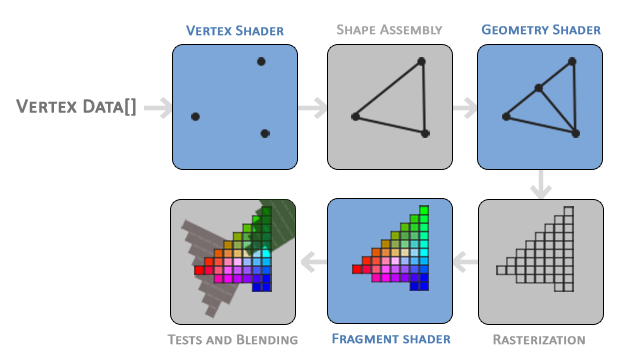
\includegraphics[scale=2]{res/oglpipeline.png}
    \caption[\acrshort{OpenGL}-Pipeline]{\acrshort{OpenGL}-Pipeline\footnotemark}
    \label{fig:opengl-pipe}
\end{figure}
\footcitetext{ogl-pipeline-logl}

\subsection{Vulkan}
Vulkan wird als Nachfolger von \acrshort{OpenGL} angesehen. Vulkan wird ebenfalls von der Khronos Group entwickelt und vertrieben. Es wurde zuerst unter den Namen \textit{Next Generation \acrshort{OpenGL}} und \textit{glNext} vorgestellt aber im Februar 2016 als Vulkan 1.0 veröffentlicht. Es ist abgeleitet von einer Grafik-\acrshort{API} von AMD namens AMD Mantle. Es bietet durch seine Low-Level-Eigenschaft sehr viel Optimierungspotenzial für den Programmierer. Dies bringt aber auch Nachteile mit sich, bezüglich der Fehleranfälligkeit und des programmiertechnischen Aufwandes.\footcite{vktut-intro} Vulkan wird seiner Stellung als Nachfolger von \acrshort{OpenGL} jedoch durch diese Optimierbarkeit sehr gerecht. Die heutigen Spiele und Grafikapplikationen werden immer realistischer und rechentechnisch viel anspruchsvoller. Durch das immense Parallelisierungspotenzial der Computation auf Grafikkarten werden solche \acrshort{API}'s immer wichtiger. Der Bedarf für High Performance Grafik- und Compute-\acrshort{API}'s ist da. Vulkan hat im Gegensatz zu \acrshort{OpenGL} die Möglichkeit, auf mehreren \acrshort{CPU}-\glspl{Thread} zu laufen. Dadurch, dass moderne Central Processing Unit's (\acrshort{CPU}'s) ebenfalls immer mehr Kerne bekommen, sind diese \gls{Multithreading}-Kapazitäten von enormer Bedeutung und stellen den Hauptvorteil gegenüber \acrshort{OpenGL}. Vulkan ist eine sehr tief liegende \acrshort{API}. Das bedeutet, dass der Programmierer sehr viel mehr Arbeit zu erledigen hat als bei \acrshort{OpenGL}, welches höher abstrahiert und vereinfacht ist. Vulkan ist ebenfalls plattformübergreifend, jedoch noch nicht so weit verbreitet wie \acrshort{OpenGL}.\footcite{khronos-vulkan}

\subsubsection{Funktionsweise von Vulkan}
Vulkan funktioniert im Prinzip gleich wie \acrshort{OpenGL}. Auch Vulkan macht Gebrauch von Präfixen: Jeder Vulkan-Befehl beginnt mit \textit{vk*}. Auch bei Vulkan gibt es die Pipeline. Diese sieht durch die Low-Level-Eigenschaft der \acrshort{API} allerdings wesentlich komplizierter aus, wie in Abbildung \ref{fig:vk-pipe} dargestellt ist. Es gibt viel mehr Möglichkeiten, \gls{Shader} zu definieren. Unter anderem gibt es bei Vulkan Tessellation und Compute \gls{Shader}. Mittlerweile kennt \acrshort{OpenGL} das Prinzip des Tesselation \gls{Shader}s seit Version 4.0 auch.\footcite{oglwiki-tessellation} Die tiefliegende Verbundenheit mit der Computerarchitektur zeigt sich bei Vulkan auch darin, dass der Programmierer viele interne Objekte selber erstellen und zerstören muss. Während in \acrshort{OpenGL} alles intern gehandhabt wird, muss man sich bei Vulkan um eine Instance, ein Physical und Logical Device, ein Surface und einige weitere spezialisierte Dinge bemühen, bevor überhaupt etwas sichtbar ist. Weiterhin funktioniert Vulkan durch sogenannte \textit{Command Buffer}. Dies sind Ansammlungen von Befehlen, welche zuerst aufgenommen und in den Command Buffer geschrieben werden müssen und erst auf ein separates Kommando auf einer \textit{Queue} auf der Grafikkarte ausgeführt werden. Eine Queue muss man sich wie einen Prozessorkern bei der \acrshort{CPU} vorstellen. Es können Ressourcen zwischen Queues geteilt und Informationen ausgetauscht werden, damit das Programm schneller läuft. Im Prinzip funktioniert das Ganze wie \gls{Multithreading}. Jeder Zugriff auf ein Objekt muss synchronisiert werden, speziell wenn mehrere Queues auf dasselbe Objekt zugreifen. Das heisst, Vulkan führt seine Command Buffer asynchron auf der GPU aus. Dies bringt einige Vorteile mit, zieht aber auch Unannehmlichkeiten nach sich. Hauptvorteil davon ist, dass der Vulkan Treiber seine Ressourcen im Voraus allozieren und reservieren kann. Der grosse Nachteil davon ist allerdings, dass der Programmierer Vulkan-Objekte zwischen den Queues synchronisieren muss. Dies macht die Sache wesentlich komplizierter. Hinzu kommt noch eine weitere Schwierigkeit: Da bei Vulkan viel mit Buffern, Pointern und internen Objekten gearbeitet wird, kann bei jedem einzelnen Schritt etwas falsch laufen. Zum Beispiel gibt man aus Versehen einen Nullpointer oder eine fragwürdige Eingabe ein. Damit wird dann z.B. ein internes Objekt erstellt, welches durch die Eingabe ungültig ist. Vulkan direkt hat aber keine Möglichkeit Informationen zur Konsole auszugeben und dem Programmierer dadurch das Debuggen zu vereinfachen. In einem solchen Fall würde das Programm einfach abstürzen, ohne Debug-Informationen auszugeben. Das heisst, es kann zu jedem Zeitpunkt an \textit{irgendetwas} scheitern und der Programmierer hat nicht die geringste Ahnung, woran. Da sich so nur sehr schwer fähige Programme erstellen lassen, hat die Vulkan-Community die sogenannten \textit{Validation Layers} entwickelt. Diese funktionieren als Kontrollobjekte, welche sämtliche Eingaben des Programmieres auf Validität überprüfen. Gibt der Programmierer etwas ungültiges ein, so schlagen diese Alarm und melden zurück, was mit welchem Objekt nicht stimmt. Da der Vulkan-Code über seine Command-Buffer asynchron auf der Grafikkarte ausgeführt wird, ist dies allerdings nicht allzu hilfreich. Aber es ist ein Anfang, welcher wenigstens einen Hinweis gibt, in welcher Richtung das Problem gelagert sein könnte.
\begin{figure}[ht]
    \centering
    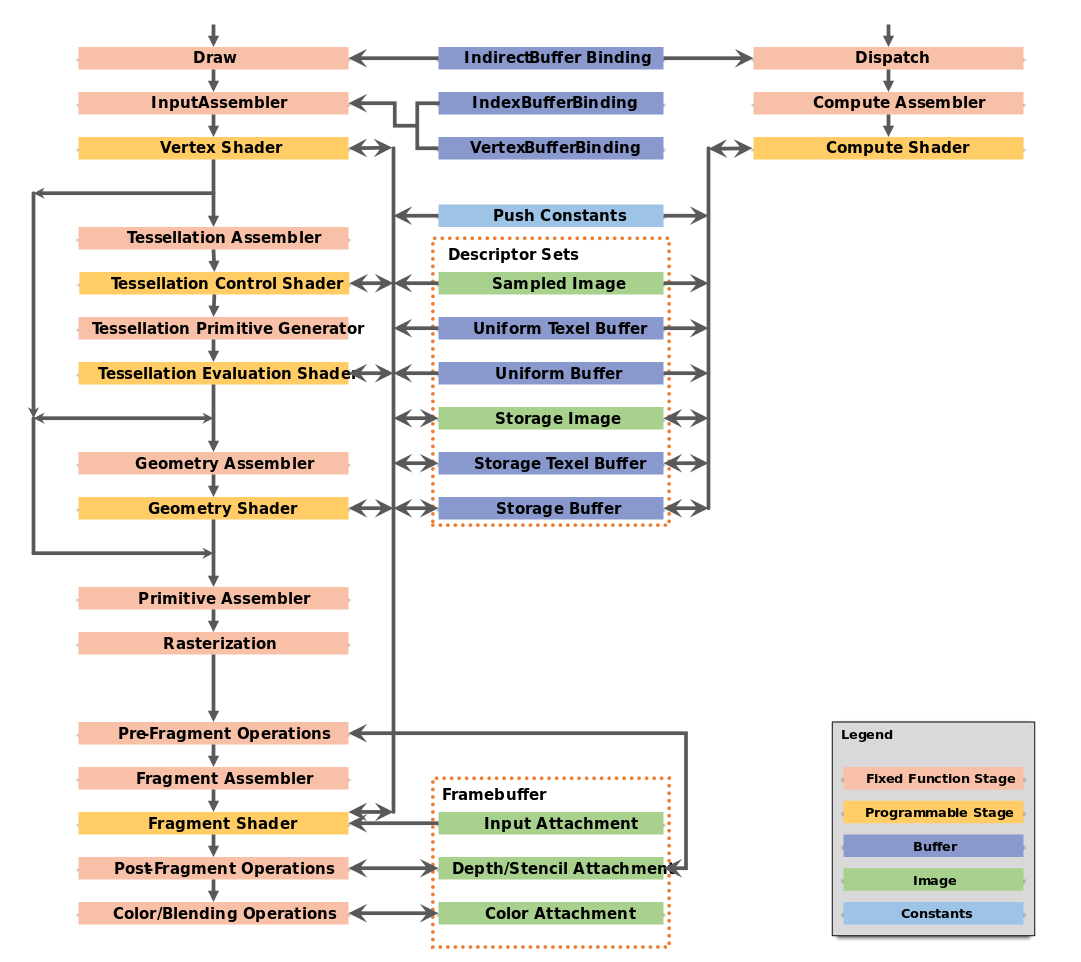
\includegraphics[scale=0.5]{res/vkpipeline1.png}
    \caption[Vulkan-Pipeline]{Vulkan-Pipeline\footnotemark}
    \label{fig:vk-pipe}
\end{figure}
\footcitetext{vk-pipeline-vkspec}
Vulkan hat eine weitere Eigenart, welche \acrshort{OpenGL} nicht hat: Es arbeitet intern sehr viel mit Structures von C/C++. Während bei \acrshort{OpenGL} z.B. Flags direkt als Funktionsparameter übergeben werden, werden bei Vulkan oft Structs leer initialisiert und dann mit Informationen gefüllt. Für viele Objekte, welche zwangsweise erstellt werden müssen, existiert ein sogenanntes \textit{Create Info Structure}. Dieses beinhaltet alle nötigen Informationen zur korrekten internen Erstellung des Objektes. Nachdem das Create Info Struct korrekt ausgefüllt ist, folgt der Befehl zur tatsächlichen Erstellung des Objektes. Diese Befehle haben immer denselben Aufbau: Der Befehl lautet \textit{vkCreate*} + das Objekt, das zu erstellen ist. Dann folgen die Parameter, wovon der erste immer das Vulkan Logical Device ($\widehat{=}$ Grafikchip) ist. Des Weiteren folgt immer der Vulkan Memory Allocator und das sogenannte \textit{Handle} des Objektes, welches man erstellen möchte, als Referenz, sodass Vulkan in dessen Speicheradresse schreiben kann. Ein Handle ist ein Datentyp von Vulkan, welcher der \acrshort{API} genau sagt, welches Objekt intern damit gemeint ist.  Auf das Objekt wird immer über das Handle zugegriffen. Der Befehl zur Erstellung gibt immer direkt einen \textit{VkResult}-Statuscode zurück, welcher angibt, ob bei der Erstellung des Objektes irgendetwas schief gelaufen ist. In Anhang D kann so eine Erstellung eines Vulkan-Objektes mit Hilfe des Create Info Structs eingesehen werden. Vulkan-Structs haben immer den Parameter \textit{sType}, welcher für den sogenannten \textit{VK\_STRUCTURE\_TYPE} steht. Dieser muss zwingend immer korrekt gesetzt werden und existiert aus dem folgenden Grund: Structs in C/C++ sind effektiv nur direkt hintereinanderliegende Variablen auf dem Speicher. Vulkan intern sieht nur das lineare Layout des Speichers. Das heisst, für Vulkan ist nur Speicheradresse nach Speicheradresse sichtbar. Es weiss nicht, wo ein Struct beginnt und wo es aufhört. Deswegen muss Vulkan dies mitgeteilt werden. Über den VK\_STRUCTURE\_TYPE weiss Vulkan um was für ein Objekt/Struct es sich handelt. Ausserdem können Erweiterungen so einfacher in Vulkan integriert werden, da diese dann keine Vulkan-Funktion komplett neu definieren müssen, sondern einfach ein Alias des Structures mit einem andere Structure Type angeben können. Eine weitere Besonderheit von Vulkan ist, dass die in \acrshort{GLSL} geschriebenen \gls{Shader} zuerst in \textit{SPIR-V}-Format kompiliert werden müssen, bevor sie gebraucht werden können. Die Kompilierung passiert bei \acrshort{OpenGL} zur Runtime, bei Vulkan zur separaten Compile-Time.

\subsection{Direkter Vergleich}
Da Vulkan so gesehen der direkte Nachfolger von \acrshort{OpenGL} ist, gibt es hier einige Dinge, welche verglichen werden können. Der Vergleich wird tabellarisch gemacht. Tabelle \ref{tab:comparison} stellt einen Vergleich bezüglich gewissen Kriterien zwischen den beiden \acrshort{API}'s her.
\begin{table}[ht]
    \centering
    \caption[Vergleich von Vulkan und \acrshort{OpenGL}]{Vergleich von Vulkan und \acrshort{OpenGL}}
    \bigbreak
    \begin{tabular}{|c||c|c|}
        \hline
        \multicolumn{3}{|c|}{Implementation} \\
        \hline
        \hline
         & \acrshort{OpenGL} & Vulkan \\
        \hline
        Aufwand & niedrig/mittel & sehr hoch \\
        Komplexität & mittel & sehr hoch \\
        Abstraktionsgrad & tief & hoch \\
        Fehleranfälligkeit & tief & hoch \\ 
        Debugmöglichkeiten & internes Error-Callback & eigenes Debug-Callback \\ & & durch externe Validation Layers \\
        Optimierungsmöglichkeiten & eher wenige & sehr viele \\
        Parallelisierungsgrad & nur teilweise auf GPU & sehr hoch \\
        \gls{Multithreading} & sehr eingeschränkt möglich & komplex, aber gut umsetzbar \\ & mit eher kleinem Ertrag & mit grossen Verbesserungen \\
        Lerneffekt über 3D-\gls{Rendering} & mittel & sehr genau und vertieft \\
        Programmiertechnisches Vorwissen & nicht fordernd & eher fordernd (moderne Standards) \\
        Plattformen & weitgehend unterstützt & nicht überall unterstützt, da sehr neu \\
        \hline
        \multicolumn{3}{c}{} \\
        \hline
        \multicolumn{3}{|c|}{Grafische Features} \\
        \hline
        \hline
         & \acrshort{OpenGL} & Vulkan \\
        \hline
        MultiSampling AntiAliasing & keine Angaben & bis zu 64-fach \\
        Depth-Testing & ja & ja \\
        Stencil-Testing & ja & ja \\
        Blending & ja & ja \\ 
        \gls{Face}-Culling & ja & ja \\
        Eigener Framebuffer & optional & zwingend \\
        Texturen und Sampler & 1D, 2D und 3D & 1D, 2D und 3D \\
        Instancing & ja & ja \\
        Normal und Parallax-Mapping & ja & ja \\
        Schatten & ja & ja \\
        HDR & ja & ja \\
        Ambient Occlusion & ja & ja \\
        Gamma Correction & ja & ja \\
        \hline
    \end{tabular}
    \label{tab:comparison}
\end{table}
\pagebreak
\begin{table}[ht]
    \begin{tabular}{|c||c|c|}
        \hline
        \multicolumn{3}{|c|}{Leistung} \\
        \hline
        \hline
         & \acrshort{OpenGL} & Vulkan \\
        \hline
        \glspl{Frametime}/\acrshort{FPS} & top & top \\
        Auslegung & Graphics & Graphics \& Compute \\
        Flüssige Darstellung & nicht immer & eher oft \\
        Probleme & Teilweise Screen-Tearing & Je nach \textit{VK\_PRESENT\_MODE} \\
         & Stockend unter \gls{Linux} & kann Screen Tearing auftreten \\
         & V-Sync nicht deaktivierbar unter \gls{Linux} & V-Sync nicht deaktivierbar unter \gls{Linux} \\
        \hline
    \end{tabular}
\end{table}
\bigbreak
Wie aus der Tabelle hervorgeht, haben die \glspl{Engine} in etwa dieselben grafischen Features. Lediglich bei der Implementation gibt es grosse Unterschiede und Vulkan steht im ersten Moment nicht allzu gut da. In erster Linie liegt dies daran, dass \acrshort{OpenGL} kontinuierlich aktualisiert und optimiert wurde. Deswegen konnte \acrshort{OpenGL} seine Einfachheit gegenüber Vulkan behalten und dabei dieselben Leistungen erzielen. Wie schon zuvor erwähnt ist Vulkan viel hardware-näher als \acrshort{OpenGL}. Dies lässt sich auch aus der Tabelle herauslesen. Weiter ist klar erkennbar, dass es von den grafischen Features keine erkennbaren Unterschiede gibt. Bei der Leistung sticht Vulkan klar heraus, da es eigentlich immer flüssig läuft. \acrshort{OpenGL} kommt bei grossen Buffern und vielen Objekten schnell mal ins Schwitzen. Durch Parallelisierung ist dies Vulkans Hauptvorteil.\par
Dass V-Sync unter Linux nicht deaktivierbar ist, liegt bei den Implementationen entweder an der Windowing-Library \acrshort{GLFW} oder dem Windowing-System des Betriebssystemes und somit nicht direkt an den \acrshort{API}'s.\par 
Der \textit{VK\_PRESENT\_MODE} legt fest, wie ein Bild angezeigt wird, nachdem es gerendert wurde. Als Beispiel gibt es den \textit{VK\_PRESENT\_MODE\_FIFO\_KHR}. FIFO steht dabei für \textit{first in, first out}. Vulkan wartet bis der Bildschirm zum Darstellen des neuen \glspl{Frame} bereit ist und zeigt dieses erst dann. Dabei kann kein Screen Tearing auftreten, da dieses mit unterschiedlichen Aktualisierungs- und Darstellungsfrequenzen des Framebuffers und des Bildschirms zu tun hat. Der \textit{Framebuffer} ist eine Speicheransammlung im High-Performance-Arbeitsspeicher auf der Grafikkarte, in welche das aktuell gerenderte Bild geschrieben wird, bis es angezeigt werden kann. Tearing tritt dann auf, wenn der Computer beginnt, das gerenderte Bild aus dem Framebuffer zu lesen und zum Bildschirm zur Darstellung zu senden, aber mitten in diesem Prozess des Herauslesens bereits das neue \gls{Frame} hineingeschrieben wird. Dadurch zeichnet sich eine ganz klare Linie zwischen dem alten und dem neuen \gls{Frame} ab; das Bild \textit{reisst} (engl. \textit{to tear}, 'reissen'). Dies wird als Störartefakt bezeichnet und kann durch eine Synchronisation der Frequenzen behoben werden. Dies ist im Prinzip das, was V-Sync macht. Bei den Applikationen wurde für die Tests \textit{VK\_PRESENT\_MODE\_MAILBOX\_KHR} benutzt, welcher mit Tearing zu kämpfen hat und kein V-Sync besitzt. Jedoch wurde die Aktualisierungsfrequenz des Framebuffers unter Linux automatisch trotzdem mit der des Bildschirms synchronisiert. Dies konnte nicht ausgeschalten werden. Ursachen dafür wurden nicht weiter abgeklärt, da es vermutlich nicht mehr direkt mit den \acrshort{API}'s zu tun hat.

\newpage
\section{Progammierung und Implementation}

\subsection{Entwicklungsumgebung}
Als primäre Entwicklungsumgebung wurde Microsoft Visual Studio Community 2017 (und später Microsoft Visual Studio Community 2019), welches in der Community-Edition Free-Ware ist, unter Windows 10 verwendet. Microsoft Visual Studio Community bringt eine vollkommene C++-\acrshort{IDE}, d.h. \gls{Compiler}, \gls{Debugger} und \gls{Texteditor} in einem. In dieser Umgebung wurde ein Grossteil der Vulkan-Applikation, welche gegenwärtig rund 8'500 Zeilen Quellcode umfasst, geschrieben. Später in der Entwicklung wurde komplett umgestellt auf Seiten der Entwicklungsumgebung: Da die beiden Applikationen grundsätzlich plattformübergreifend programmiert wurden und nur wenige \glspl{Tweak} nötig waren, um die Software unter \gls{Linux} kompilieren zu können, wurde dies dann auch gemacht. Es wurde unter \gls{Debian} (genauer: Ubuntu 18.04/\gls{Linux} Mint 19.2) mit Microsoft's allgegenwärtigem Visual Studio Code weitergearbeitet. Microsoft Visual Studio Code ist keine \acrfull{IDE} mehr, sondern nur noch ein reiner \gls{Texteditor}. Dies bedeutet für den Entwickler, dass er auf andere \gls{Compiler} und \gls{Debugger} zurückgreifen muss. \gls{Debian} bietet die meist bereits vorinstallierte \acrfull{gcc} mit g++, dem \gls{Compiler} für C++. Als \gls{Debugger} wurde der ebenfalls meist schon vorinstallierte \acrfull{gdb} verwendet.

\subsubsection{Verwendete Tools und Hilfsmittel}
Für die Entwicklung der beiden Applikationen wurden mehrere \glspl{Tool} verwendet, die dem Entwickler die Arbeit sehr vereinfachen. Als \acrfull{VCS} wurde Git in Kombination mit der Source-Code-Sharing-Plattform \gls{GitHub} verwendet. Dies erlaubt einfaches Zurückspringen zu alten Versionen und \gls{Tracking} jeder einzelner Änderung. Es bringt gute Möglichkeiten der Zusammenarbeit, wenn mehrere Entwickler am selben Projekt arbeiten würden, was bei diesen zwei Projekten (bis auf eine kleine Ausnahme) nicht der Fall war. Ausserdem wurde GitKraken als Git-\acrshort{GUI}-Client benutzt, da Git eigentlich hauptsächlich für die Konsole/das Terminal ausgelegt ist. Zusammen mit \gls{GitHub} wurde die \acrfull{CI}-Lösung Travis \acrshort{CI} eingesetzt. \acrshort{CI}-Lösungen sind dafür zuständig, bei einer Änderung/Neuerung im Quellcode des Projektes, immer dieselben Tests durchzuführen, um sicherzustellen, dass die Software nach dieser Änderung weiterhin so funktioniert, wie sie sollte.\par
Vor dem Wechsel zu \gls{Linux} wurde nur die Microsoft Visual Studio-\acrshort{IDE} verwendet, da diese alles notwendige an einem Ort bot. Unter \gls{Linux} wurden dann, wie schon gesagt, Visual Studio Code und g++ mit \acrshort{gdb} benutzt. Ausserdem wurde mit Processing 3 eine kleine Doppelpendel-Simulation geschrieben, die dazu diente, die Bewegungsgleichungen und Formeln für das Pendel zu testen.

\subsubsection{Verwendete Bibliotheken}
In den Applikationen wurde nicht alles von Hand geschrieben. Für gewisse Teilbereiche wurden Bibliotheken benötigt, da die Zeit und teilweise das Knowhow fehlten, gewisse Dinge selber zu programmieren. Folgende Libraries wurden verwendet:
\begin{itemize}
    \item \acrfull{ASSIMP}
    \item \acrfull{GLFW}
    \item tinyobjloader
    \item stb\_image.h
    \item \acrfull{SDL}
    \item \acrfull{GLM}
    \item GLAD
\end{itemize}
\acrshort{ASSIMP} bietet sehr schnelles und zuverlässiges Laden von 3D-Modellen vieler verschiedener Formate. \acrshort{GLFW} als Windowing-Library bietet alles Notwendige für ein Applikationsfenster und \acrshort{OpenGL}- resp. Vulkan-Kontexte. Tinyobjloader ist eine zweite Model-Loading-Bibliothek, welche zuerst als einfachere Variante implementiert wurde, später jedoch mit einigen 3D-Modellen nicht mehr funktionierte. Die Header-Only-Library std\_image.h dient dem Laden von Texturen aus den Modell-Dateien und sonstigen Bilddateien wie dem Icon und dem Ladebildschirm der Applikation. \acrshort{SDL} ist eine weitere Windowing-Library, welche \acrshort{OpenGL}/Vulkan-Kontexte erzeugen kann, aber primär für den Ladebildschirm gebraucht wurde. \acrshort{GLM} ist eine Bibliothek für lineare Algebra und Vektorgeometrie. Dies hätte auch ohne Probleme selber umgesetzt werden können, aber aufgrund der Zeitknappheit wurde darauf verzichtet. GLAD wurde nur für die \acrshort{OpenGL}-Applikation verwendet. Es dient dazu die Function-Pointer für die \acrshort{OpenGL}-Funktionen zu setzen, da diese sonst nicht bekannt wären. Alle Libraries sind OpenSource und plattformübergreifend. Teilweise mussten die Libraries selber kompiliert werden, was insofern ein Problem darstellte als dass diese meistens nur für 32-bit, die Applikationen jedoch auf 64-bit-Architekturen ausgelegt waren. Nach einiger Zeit wurde allerdings auch diese Hürde überwunden und beide Applikationen funktionierten seitdem auf 64-bit-Architekturen.

\subsection{OGL}
Die Entwicklung der \acrshort{OpenGL}-Applikation verlief problemlos. Da zuerst die Vulkan-\gls{Engine} geschrieben wurde, konnten bei \acrshort{OpenGL} grosse Teile des Quellcodes 1 zu 1 kopiert werden. Beispiele dafür wären das Kamerasystem, das Model-Loading-System, der Startbildschirm, die eigens erstellte Logginglösung und die grundsätzliche Struktur der Applikationen. Sie sind in sich sehr ähnlich aufgebaut; der grösste Unterschied zwischen der Vulkan- und der \acrshort{OpenGL}-Implementation besteht darin, dass bei Vulkan die $y$-Achse ein negatives Vorzeichen hat. Da sehr modular und im Hinblick auf Kompatibilität zwischen beiden \glspl{Engine} gearbeitet wurde war es ein leichtes, grosse Teile einfach zu übernehmen. Dadurch, dass \acrshort{OpenGL} an sich nicht sehr kompliziert ist und sehr schnell Resultate, welche sehr vorzeigbar sind, erarbeitet werden können, dauerte die Entwicklung mit \acrshort{OpenGL} nur ungefähr vier Arbeitstage und lieferte hierbei dieselben grafischen Leistungen wie die Vulkan-Applikation. Die nennenswertesten davon umfassen MipMapping, MultiSampling AntiAliasing, Color-Blending und Depth-Testing. \par
Grundsätzlich unterstützt \acrshort{OpenGL} kein \gls{Multithreading}. Das heisst, es lässt nativ keine Parallelisierung durch den Programmierer zu, sondern möchte alles \acrshort{API}-intern handhaben und selbst optimieren. Dies bedeutet grundsätzlich längere Lade- und Startzeiten der Applikationen mit \acrshort{OpenGL}, da diese nur mit einem Thread gleichzeitig Assets laden können. Unter Assets versteht man generell Modelle, Texturen, Audiodateien und dergleichen.

\subsection{VK}
Das Development der Vulkan-\gls{Engine} verlief nicht ganz so problemlos, vor allem da diese zuerst geschrieben wurde. Das bedeutete, die ganzen Systeme, welche bei \acrshort{OpenGL} einfach übernommen wurden, mussten hier zuerst erarbeitet und entwickelt werden. Dass hierbei viele kleine aber feine Bugs und Fehler entstehen, war erwartbar. In welcher Grössenordnung dies geschieht, war nicht vorauszusehen und es wurde definitiv nicht in dem schlussendlichen Ausmass erwartet. Dies führte zu grossen Verzögerungen und die \glspl{Engine} mussten auf einige eigentlich geplante Features verzichten. Da der Programmierer bei Vulkan sehr low-level arbeitet, muss er viel mehr selber machen als bei höheren \acrshort{API}'s wie \acrshort{OpenGL}. Dies führt einerseits zu einer grösseren Freiheit für Leistungsoptimierungen, andererseits zu einem sehr viel grösseren Aufwand für dasselbe Ergebnis. Man schaue sich die rohen Zahlen an: Bei \acrshort{OpenGL} betrug die Anzahl Zeilen Quellcode in der finalen Form ca. 3'500, bei Vulkan etwa 8'500. Dass bei rund 5'000 Zeilen mehr Code viel mehr Fehler entstehen können, ist zu erwarten. 
Insbesondere gab es ein Problem, welches über mehrere Wochen bestand: Es wurden Texturen nicht richtig dargestellt. Es wurde alles mehrmals überprüft: Texturkoordinaten, Texturdateien, die \gls{Shader}, die Mappings auf das Modell... Nichts schien zu helfen, nicht eimal das Update auf die Vulkan Spec-Version 1.1.114.0. Dann wurden die Lighting-Berechnungen eingebaut und plötzlich waren die Artefakte einfach weg, wofür bis heute keine rationale Erklärung gefunden wurde. Ein weiteres Problem an welchem lange gearbeitet wurde stand im Zusammenhang mit der Asynchronität von Vulkans Ausführung auf der Grafikkarte. Da nicht bekannt war, welches Modell gerade durch die Pipeline und die \gls{Shader} gepumpt wurde, war zwangsweise ebenfalls nicht bekannt, wann welche Model-Matrix zu den \gls{Shader}n gesendet werden musste. Die einfachste Lösung boten die sogenannten \textit{Push Constants}. Push Constants dienen dazu, an einem bestimmten Punkt der Ausführung eines Command Buffers einen Wert zu den \gls{Shader}n hochzuladen. Somit kann genau dann, wenn ein bestimmtes Model die \gls{Shader} Stages durchläuft, ein Wert hochgeladen werden. An sich sind Push Constants sehr schnelle und performancegünstige Lösungen, um kleinere Datenmengen hochzuladen. Push Constants müssen laut der Vulkan \acrshort{API} Spezifikation immer mindestens 128 Byte unterstützen.\footcite{push-constant-vkspec} Dies passt perfekt für eine $4\times4$-Matrix aus 32-bit \glspl{Float} wie die Model-Matrix eine ist: $4 \cdot 4 \cdot 32$ Bit $= 512$ Bit $\widehat{=}$ 64 Byte. Die Model-Matrix muss also zwangsweise auf jedem System immer durch Push Constants hochgeladen werden können. Das Wörtchen 'Constant' jedoch birgt ein Problem: Die Model-Matrix wäre konstant, also jedesmal dieselbe. Das Modell würde sich nicht bewegen, rotieren oder sonst irgendwie verändern können. Um diese konstante Qualität wegzunehmen wurden die Command Buffer jedes \gls{Frame} neu aufgenommen und somit implizit auch die \textit{Descriptor Sets}, welche als Übermittler von Daten an \gls{Shader} agieren, neu erstellt. Dies führt zu einem dramatischen Performanceverlust. Besser wäre es gewesen, einen grösseren Uniform Buffer hochzuladen und dann über eine Push Constant in ein Array an Model-Matrizen zu indexieren. Dies wurde jedoch absichtlich nicht umgesetzt, da es erstens nicht direkt funktionieren wollte und es zweitens Nachteile nach sich zieht: Entweder es wird ein dynamischer Uniform Buffer eingführt (kompliziert), oder es gibt eine Obergrenze an Modellen, welche dargestellt werden können. Deswegen wurde dies vorerst nicht umgesetzt, hauptsächlich wegen des Zeitdrucks. Die Leistung der Vulkan-\gls{Engine} wurde aber nicht völlig vernachlässigt. Es wurde lange Zeit damit zugebracht, \gls{Multithreading} für das Asset-Loading einzubauen. Dort gab es lange Probleme mit der Synchronisation, da zeitweise auf bis zu 12 \glspl{Thread} gleichzeitig gearbeitet wurde. Das System funktioniert über einen Handler-Thread und 12 Worker-\glspl{Thread}. Der Handler-Thread pusht dabei neu eintreffende Ladeaufträge zu einem Warteschlangen-Objekt der Standardbibliothek von C++ und der erste Worker-Thread, der frei ist, nimmt immer das vorderste Element dieser \textit{std::queue} (engl. \textit{queue}, 'Warteschlange'). So kann die \acrshort{CPU} im Zusammenspiel mit Vulkan optimal ausgenutzt werden. Das Problem ist nur, dass Vulkan den Zugriff mehrerer \glspl{Thread} auf gewisse Objekte und Parameter selbst intern mit seinen \textit{VkFence}'s, \textit{VkSemaphore}'s oder \textit{VkMemoryBarrier}'s synchronisiert und den Zugriff auf andere nicht. Dabei ist in der Vulkan Spezifikation genau definiert welche Parameter bei welchen Funktionen vom Programmierer mit externen Synchronisationsobjekten wie STL's \textit{std::mutex} synchronisiert werden müssen.\footcite{vkspec-multithreading}

\subsection{Lizensierung der Software}
Beide Applikationen/Projekte sind unter der \textit{GNU General Public License v3.0} lizensiert. In der Kurzfassung heisst dies, der Source-Code darf unter Angabe von Copyright, Quelle und Einbindung derselben Lizenz ohne jegliche Haftung oder Garantie des Entwicklers für kommerzielle, private und patentierte Zwecke genutzt werden. Die Software darf unter Angabe der Änderungen modifiziert und veröffentlich werden. Für die verwendeten Bibliotheken existieren Lizenzen innerhalb des Source-Codes oder wo nötig in separaten Dateien. Die Lizenzen der Libraries erlauben allesamt die Nutzung und Veröffentlichung in eigenen Projekten.


\newpage
\section{Das Doppelpendel}

\subsection{Was ist ein Doppelpendel?}
Ein Doppelpendel ist im physikalischen Sinne ein beliebtes Modell zur Darstellung von determinis-tisch-chaotischen Prozessen. Das Pendel ist deterministisch, weil die Bewegungsgleichungen bekannt und berechenbar sind. Es ist chaotisch, weil sich das Doppelpendel bei kleinsten Änderungen der Startbedingungen drastisch anders verhält. In den Grundzügen ist ein Doppelpendel sehr einfach: An die Masse $m_{1}$ eines mathematischen Pendels der Länge $\ell_{1}$ wird ein weiteres mathematisches Pendel mit Masse $m_{2}$ und Länge $\ell_{2}$ gehängt. $\theta_{1}$ und $\theta_{2}$ bilden die Auslenkungswinkel gegenüber der Vertikalen. Die Verbindungsstücke sind starr, d.h. die Längen $\ell_{1}$ und $\ell_{2}$ sind konstant. Abbildung \ref{fig:dp-graphic} veranschaulicht den generellen Aufbau eines Doppelpendels.
\begin{figure}[ht]
    \centering
    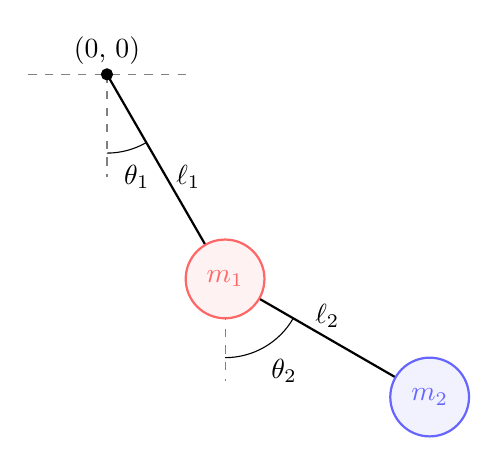
\begin{tikzpicture}
        \draw[gray, dashed] (-1,0) -- (1,0);
        \draw[gray, dashed] (0,0) coordinate (a) -- (0,-1.3) coordinate (b);
        \filldraw[black] (0,0) circle (2pt) node[anchor=south] {(0, 0)};
        \draw[black, thick] (0,0) -- (1.5,-2.59807621135) coordinate (c) node[midway,anchor=west] {$\ell_{1}$};
        \draw[gray, dashed] (c) -- (1.5,-3.89807621135) coordinate (d); 
        \draw[black, thick] (c) -- (4.09807621135,-4.09807621135) coordinate (e) node[midway,anchor=south] {$\ell_{2}$};
        \draw[black] (0, -1) arc (-90:-60:1);
        \draw[black] (1.5,-3.59807621135) arc (-90:-30:1);
        \node[] at (0.38,-1.3) {$\theta_{1}$};
        \node[] at (2.25,-3.77)  {$\theta_{2}$};
        \filldraw[color=red!60, fill=red!5, thick] (c) circle (0.5) node {$m_{1}$};
        \filldraw[color=blue!60, fill=blue!5, thick] (e) circle (0.5) node {$m_{2}$};
    \end{tikzpicture}
    \caption[Schema eines Doppelpendels]{Schema eines Doppelpendels}
    \label{fig:dp-graphic}
\end{figure}

\subsection{Wieso ein Doppelpendel?}
Da sich diese Arbeit grundsätzlich auf \gls{Floating-Point}-Arithmetik bezieht, welche durch z.B. Rundungsfehler sehr schnell sehr ungenau werden kann, ist ein deterministisch-chaotisches System perfekt, um ebendies zu visualisieren. Da das Programmieren von kompetenten Render-\glspl{Engine} eine sehr aufwändige und komplizierte Angelegenheit ist, wurde auf ein einfach umzusetzendes deterministisch-chaotisches System gesetzt: das Doppelpendel. Andere Möglichkeiten wären zum Beispiel ein Drehpendel gewesen, oder sogar eine Wellensimulation, welche den berüchtigten \acrfull{IFFT}-Algorithmus benötigt hätte. Letzteres wäre jedoch mit grossem Aufwand und viel Zeit verbunden gewesen, welche für diese Arbeit nicht zur Verfügung standen.

\subsection{Physik hinter dem Doppelpendel}
\subsubsection{Variablen und Parameter}
Die Variablen der beiden Pendel werden indiziert, d.h. für das erste Pendel Index 1, für das zweite Index 2. In den Formeln und Herleitungen werden folgende Variablen verwendet:
\begin{itemize}
    \item $x_{1, 2} = $ horizontale Position der Pendelmasse
    \item $y_{1, 2} = $ vertikale Position der Pendelmasse
    \item $\theta_{1, 2} = $ Winkel des Pendels gegenüber der Vertikalen, Gegenuhrzeigersinn ist positiv
    \item $\ell_{1, 2} = const. = $ Länge des starren Verbindungsstückes
    \item $m_{1, 2} = const. = $ Masse des Pendels
    \item $r_{1, 2} \propto m_{1, 2} = const. = $ Radius der Pendelmasse
    \item $g = const. = $ Ortsfaktor / Gravitationsbeschleunigung
\end{itemize}

\subsubsection{Voraussetzungen und Annahmen}
Wie berechnen sich die Positionen der beiden Massen relativ zum Ursprung? Für die folgende Herleitung werden gewisse Annahmen gemacht, resp. gewisse Voraussetzungen festgelegt:
\begin{itemize}
    \item Es gibt keine Reibung und somit auch keinen Luftwiderstand.
    \item Die Verbindungsstücke mit Länge $\ell_{1}$ und $\ell_{2}$ haben keine Masse.
    \item Die Massen $m_{1}$ und $m_{2}$ sind konstant und werden als Massepunkte betrachtet.
    \item Die Radien $r_{1, 2}$ der Kugeln sind proportional zur Masse der Kugel.
    \item Der Drehpunkt des ersten Pendels liegt in $(0, 0)$.
    \item Die $y$-Achse ist nach oben steigend, die $x$-Achse nach rechts. Die Achsen stehen im Ursprung senkrecht aufeinander und haben dieselben Einheiten.
\end{itemize}

\subsubsection{Kinematik des Doppelpendels}
Zu Beginn werden erst einmal die einfachen trigonometrischen Beziehungen benutzt, um Ausdrücke für die Positionen der Pendelmassen $M_{1} (x_{1}, y_{1})$ und $M_{2} (x_{2}, y_{2})$ in Abhängigkeit zu den von der Zeit $t$ abhängigen Auslenkungswinkeln $\theta_{1} = \theta_{1}(t)$ und $\theta_{2}= \theta_{2}(t)$ zu finden. Dies wird komponentenweise gemacht. Es handelt sich somit um eine simple Umrechnung von Polar- in kartesische Koordinaten:
\begin{align}
    x_{1} &= \ell_{1} \sin{\theta_{1}} \\
    y_{1} &= -\ell_{1} \cos{\theta_{1}} \\
    x_{2} &= x_{1} + \ell_{2} \sin{\theta_{2}} \\
    y_{2} &= y_{1} - \ell_{2} \cos{\theta_{2}}
\end{align}
\bigbreak
Positionen abgeleitet nach der Zeit $t$ ergeben die jeweiligen Geschwindigkeiten:
\begin{align}
    \frac{d}{dt} x_{1} &= \frac{d\theta_{1}}{dt} \ell_{1} \cos{\theta_{1}} \\
    \frac{d}{dt} y_{1} &= \frac{d\theta_{1}}{dt} \ell_{1} \sin{\theta_{1}} \\
    \frac{d}{dt} x_{2} &= \frac{d}{dt}x_{1} + \frac{d\theta_{2}}{dt} \ell_{2} \cos{\theta_{2}} \\
    \frac{d}{dt} y_{2} &= \frac{d}{dt}y_{1} + \frac{d\theta_{2}}{dt} \ell_{2} \sin{\theta_{2}}
\end{align}
\bigbreak
Und die Geschwindigkeiten wiederum nach der Zeit abgeleitet ergeben die Beschleunigungen:
\begin{align}
    \frac{d^2}{dt^2}x_{1} &= - (\frac{d\theta_{1}}{dt})^{2} \ell_{1} \sin{\theta_{1}} + \frac{d^{2}\theta_{1}}{dt^{2}} \ell_{1} \cos{\theta_{1}} \\
    \frac{d^{2}}{dt^{2}}y_{1} &= (\frac{d \theta_{1}}{dt})^{2} \ell_{1} \cos{\theta_{1}} + \frac{d^{2}\theta_{1}}{dt^{2}} \ell_{1} \sin{\theta_{1}} \\
    \frac{d^{2}}{dt^{2}}x_{2} &= \frac{d^{2}x_{1}}{dt^{2}} - (\frac{d \theta_{2}}{dt})^{2} \ell_{2} \sin{\theta_{2}} + \frac{d^{2}\theta_{2}}{dt^{2}} \ell_{2} \cos{\theta_{2}} \\
    \frac{d^{2}}{dt^{2}}y_{2} &= \frac{d^{2}y_{1}}{dt^{2}}
    + (\frac{d \theta_{2}}{dt})^{2} \ell_{2} \cos{\theta_{2}} + \frac{d^{2}\theta_{2}}{dt^{2}} \ell_{2} \sin{\theta_{2}}
\end{align}
\bigbreak
Hierbei entspricht die Winkelgeschwindigkeit $\omega = \frac{d}{dt} \theta$ der ersten, und die Winkelbeschleunigung $\alpha = \frac{d^{2}}{dt^{2}} \theta$ der zweiten Ableitung des Winkels nach der Zeit.

\subsubsection{Mechanik des Doppelpendels}
Auf die Pendelmassen wirken Kräfte. Zum einen die Kraft der Verbindungsstücke $(F_{1, 2})$ auf die einzelnen Massen, zum anderen die Gravitationskraft. Die Idee hinter der folgenden betragsmässigen Betrachtung birgt das Aktionsprinzip resp. das zweite newtonsche Gesetz: 
\begin{align*}
    \vec{F} = m \cdot \vec{a}
\end{align*}
\bigbreak
Auf $m_{1}$ wirken die Kräfte der beiden Verbindungsstücke, also $F_{1}$ und $F_{2}$, sowie die Gravitationskraft $m_{1} \cdot (-g)$ (negatives Vorzeichen da $g$ in negative $y$-Richtung wirkt):
\begin{align}
    m_{1} \frac{d^{2}x_{1}}{dt^{2}} &= -F_{1} \sin{\theta_{1}} + F_{2} \sin{\theta_{2}} \\
    m_{1} \frac{d^{2}y_{1}}{dt^{2}} &= F_{1} \cos{\theta_{1}} - F_{2} \cos{\theta_{2}} - m_{1}g
\end{align}
\bigbreak
Auf $m_{2}$ wirken die Kräfte des Verbindungsstücks zu $m_{1}$, also $F_{2}$, und die Gravitationskraft $m_{2} \cdot (-g)$:
\begin{align}
    m_{2} \frac{d^{2}x_{2}}{dt^{2}} &= -F_{2} \sin{\theta_{2}} \\
    m_{2} \frac{d^{2}y_{2}}{dt^{2}} &= F_{2} \cos{\theta_{2}} -m_{2}g
\end{align}

\subsubsection{Bewegungsgleichungen}
Mit den Gleichungen (1) - (12) existieren drei verschiedene Arten auf die Position zu schliessen. Jedoch gibt es überall mindestens eine Unbekannte, welche auch in den Gleichungen (13) - (16) vorkommt: $\theta_{1, 2}$, $\frac{d}{dt}\theta_{1, 2}$ oder $\frac{d^{2}}{dt^{2}}\theta_{1, 2}$. Der nächste Schritt besteht also darin einen Ausdruck für $\frac{d^{2}}{dt^{2}}\theta_{1, 2}$ zu finden.\bigbreak
Die Gleichungen (15) und (16) werden nach $F_{2} \sin{\theta_{2}}$ resp. $F_{2} \cos{\theta_{2}}$ aufgelöst und in (13) resp. (14) substituiert:
\begin{align}
    m_{1} \frac{d^{2}x_{1}}{dt^{2}} &= -F_{1} \sin{\theta_{1}} - m_{2} \frac{d^{2}x_{2}}{dt^{2}} \\
    m_{1} \frac{d^{2}y_{1}}{dt^{2}} &= F_{1} \cos{\theta_{1}} - m_{2} \frac{d^{2}y_{2}}{dt^{2}} - m_{2}g - m_{1}g
\end{align}
\bigbreak
Weiter wird Gleichung (17) mit $\cos{\theta_{1}}$ und Gleichung (18) mit $\sin{\theta_{1}}$ multipliziert und gleichzeitig umgeschrieben:
\begin{align}
    F_{1} \sin{\theta_{1}} \cos{\theta_{1}} &= - \cos{\theta_{1}} (m_{1} \frac{d^{2}x_{1}}{dt^{2}} + m_{2} \frac{d^{2}x_{2}}{dt^{2}}) \\
    F_{1} \sin{\theta_{1}} \cos{\theta_{1}} &= \sin{\theta_{1}} (m_{1} \frac{d^{2}y_{1}}{dt^{2}} + m_{2} \frac{d^{2}y_{2}}{dt^{2}} + m_{2}g + m_{1}g)
\end{align}
\bigbreak
Zusammengefasst führt dies zu folgender Gleichung:
\begin{align}
    \sin{\theta_{1}} (m_{1} \frac{d^{2}y_{1}}{dt^{2}} + m_{2} \frac{d^{2}y_{2}}{dt^{2}} + m_{2}g + m_{1}g) &= - \cos{\theta_{1}} (m_{1} \frac{d^{2}x_{1}}{dt^{2}} + m_{2} \frac{d^{2}x_{2}}{dt^{2}})
\end{align}
\bigbreak
Analog wird Gleichung (15) mit $\cos{\theta_{2}}$, Gleichung (16) mit $\sin{\theta_{2}}$ multipliziert und umgeschrieben:
\begin{align}
    F_{2} \sin{\theta_{2}} \cos{\theta_{2}} &= - \cos{\theta_{2}} (m_{2} \frac{d^{2}x_{2}}{dt^{2}}) \\
    F_{2} \sin{\theta_{2}} \cos{\theta_{2}} &= \sin{\theta_{2}} (m_{2} \frac{d^{2}y_{2}}{dt^{2}} + m_{2}g)
\end{align}
\bigbreak
Was dann ebenfalls zu einer Gleichung zusammengefasst werden kann:
\begin{align}
    \sin{\theta_{2}} (m_{2} \frac{d^{2}y_{2}}{dt^{2}} + m_{2}g) &= - \cos{\theta_{2}} (m_{2} \frac{d^{2}x_{2}}{dt^{2}})
\end{align}
\bigbreak
Jetzt können die Gleichungen (21) und (24) mithilfe der Definitionen (9) bis (12) mit einem Computeralgebraprogramm gelöst werden. Somit können die folgenden Ausdrücke für $\frac{d^{2}}{dt^{2}}\theta_{1, 2}$ gefunden werden:
\begin{align}
    \frac{d^{2}}{dt^{2}}\theta_{1} &= \frac{- g (2 m_{1} + m_{2}) \sin{\theta_{1}} - m_{2}g \sin{(\theta_{1} - 2 \theta_{2})} - 2 \sin{(\theta_{1} - \theta_{2})} m_{2} ((\frac{d\theta_{2}}{dt})^{2} \ell_{2} + (\frac{d \theta_{1}}{dt})^{2} \ell_{1} \cos{(\theta_{1} - \theta_{2})})}{\ell_{1} (2m_{1} + m_{2} - m_{2} \cos{(2 \theta_{1} - 2 \theta_{2})})} \\
    \frac{d^{2}}{dt^{2}}\theta_{2} &= \frac{2 \sin{(\theta_{1} - \theta_{2})} ((\frac{d \theta_{1}}{dt})^{2} \ell_{1} (m_{1} + m_{2}) + g (m_{1} + m_{2}) \cos{\theta_{1}} + (\frac{d \theta_{2}}{dt})^{2} \ell_{2}m_{2} \cos{(\theta_{1} - \theta_{2})})}{\ell_{2} (2m_{1} + m_{2} - m_{2} \cos{(2 \theta_{1} - 2 \theta_{2})})}
\end{align}
\bigbreak
Dies sind die Bewegungsgleichungen für die Massen $m_{1}$ und $m_{2}$\footcite{dp-kinematics-website}. Hierbei handelt es sich um Differentialgleichungen. Es müssen jedoch keine komplizierten Lösungsverfahren angewendet werden, da diese Berechnungen numerisch durchgeführt werden.

\subsection{Programmatische Umsetzung}
Da es sich hierbei um nicht-konstant-beschleunigte Kreisbewegungen handelt, wurden im Quellcode pro Iteration die Winkelbeschleunigung zur Winkelgeschwindigkeit, und die resultierende Winkelgeschwindigkeit zum Winkel addiert:
\begin{minted}[linenos=true]{cpp}
float p1_theta;
float p2_theta;
float p1_vel;
float p2_vel;
float p1_acc;
float p2_acc;

void computePendulumState() {
    
    [...]
    
    p1_acc = getAccP1();
    p2_acc = getAccP2();
        
    [...]
        
    p1_vel += p1_acc;
    p2_vel += p2_acc;
    p1_theta += p1_vel;
    p2_theta += p2_vel;
    
    [...]
    
}
\end{minted}
Aber ist dies physikalisch vertretbar? Mit einem kleinen Trick, ja. Die Geschwindigkeit ist die Änderung des Ortes pro Zeit. Die Beschleunigung ist die Änderung der Geschwindigkeit pro Zeit. Dies ist praktisch die Definition der Differentialrechnung. 'Pro Zeit' $ = \Delta t = const.$ Wenn das $\Delta t$ infinitissimal klein wird, spricht man von $dt$. Es handelt sich dabei immer um dieselben Zeitabschnitte. Aber hier befinden wir uns in einer Computersimulation, wo Iterationen über eine Schleife garantiert nicht immer gleich lange dauern, und dort liegt auch das Problem. Wenn jedoch irgendwie sichergestellt wäre, dass die Iterationen immer etwa gleich lange dauern und das $\Delta t$ somit \textit{fast} konstant wäre ($\Delta t \approx const.$), könnte man dies eher vertreten. Der Trick besteht darin, dass man ein Prinzip aus der Simulationstechnik anwendet: der sogenannte Timestep. Als Timestep wird ein Verfahren bezeichnet, bei dem man in einer Iteration mehrmals dieselbe Berechnung durchführt, um gewisse Prozesse in Simulationen zu beschleunigen. Mehrere Iterationen pro Iteration der Hauptschleife helfen hier aber nicht weiter, wenn das Ziel ist, ein konstantes $\Delta t$ zu garantieren. Deshalb wird das Verfahren umgekehrt: Es werden weniger Iterationen pro Hauptschleifeniteration gemacht, und durch eine Zeitdifferenz vergleichsweise genau gezählt. Und so funktioniert es: Am Anfang der Schleife nimmt man einen Zeitstempel auf. Am Ende der Schleife schreibt man diesen in eine statische Variable, welche bei der nächsten Iteration abrufbar ist. Bei der nächsten Iteration wird der Zeitstempel am Anfang der Schleife aktualisiert. Wenn jetzt die Differenz zwischen diesem neuen Anfangszeitstempel und dem Zeitstempel der letzten Iteration grösser als z.B. $\frac{1}{60} s$ (entspricht 60 Iterationen pro Sekunde = 60 Hz) ist macht man die nächste Iteration, ansonsten wird gewartet bis die Differenz grösser ist. Hier wurde der eingebaute Timer der Windowing-Library \acrshort{GLFW} 3 \textit{glfwGetTime()} verwendet. So wird mit einer minimalen Ungenauigkeit in der Grössenordnung von einigen Nano- bis Mikrosekunden\footcite{glfwGetTimeDoc} garantiert, dass es keine nennenswerten Unterschiede beim $\Delta t$ gibt. So wurde das im Quellcode umgesetzt:
\begin{minted}[linenos=true]{cpp}
void computePendulumState() {

    double now = glfwGetTime();
    static double last = 0.0;

    if (now - last >= 1 / 60.0f) {

        [...]

        p1_acc = getAccP1();
        p2_acc = getAccP2();

        [...]

        p1_vel += p1_acc;
        p2_vel += p2_acc;
        p1_theta += p1_vel;
        p2_theta += p2_vel;
        
        [...]
        
        last = now;

    }

}
\end{minted}
Und deshalb sollten diese einfachen Additionen physikalisch gesehen kein Problem sein. All dies führt zu einer nahtlosen Simulation, welche allerdings ein Problem mit sich bringt: Die Gesamtenergie des Systems wird je nach Wahl der Startparameter über kurz oder lang gegen $\pm\infty$ gehen, da alle Störkräfte wie Reibung und Luftwiderstand vernachlässigt werden und vor allem da mit 32-bit \glspl{Float} gerechnet wird, was zu Rechenungenauigkeiten führt. Wenn die aktuelle Energie $E_{\text{tot}}$ aufgrund von Rechenungenauigkeiten über die theoretisch maximal mögliche Energie $E_{\text{max}}$ hinaussteigt, explodieren die Werte. Dies wird durch die iterative Struktur der Bewegungsgleichungen (neue Winkelbeschleunigung wird in Abhängigkeit der alten Winkelgeschwindigkeit berechnet) verstärkt. Dadurch könnte es sein, dass die Zahlen sehr schnell steigen und sehr hohe Beschleunigungen, Geschwindigkeiten und Winkel herauskommen. Nach IEEE-754-Standard können 32-bit \gls{Floating-Point}-Zahlen Werte bis maximal $(2 - 2^{-23}) \cdot 2^{127} \approx 3.4028235 \cdot 10^{38}$ darstellen. Wird versucht, einen grösseren Wert in diesen zu kleinen Speicher zu schreiben, könnte dies einen ungehandelten Buffer-Overflow zur Folge haben. Es würde somit mit ungültigen Werten weitergerechnet. Im extremsten Fall würden die Matrix-Berechnungen mit den Variablen für die Winkel, welche als 32-bit \glspl{Float} definiert wurden, Resultate liefern, die keinen Sinn machen (sog. \acrshort{NaN}'s). Das Doppelpendel würde nicht mehr dargestellt werden können. Und das Experiment zeigt, dass dem auch so ist. Mit gewissen Startwerten für Startgeschwindigkeiten, Startbeschleunigungen und Auslenkungswinkel passiert genau dies. Über kurz oder lang bauen sich die Variablen gegen $\pm\infty$ auf. Dies kann in Bruchteilen von Sekunden oder über einen längeren Zeitraum, wo man sieht wie die Rotationen der Pendel immer ekstatischer werden, geschehen. Und dann ist das Pendel plötzlich einfach weg. Dies war während der Implementation des Doppelpendels lange Zeit ein grosses Problem und hing vor allem mit einem Umrechnungsfehler von Grad- zu Bogenmass zusammen, wodurch mit viel völlig falschen Werten gerechnet wurde. Mit den richtigen Parametern lässt sich eine stabile Simulation erzeugen, welche nicht plötzlich kollabiert. Mit gewissen Startwerten für gewisse Parameter lässt sich trotzdem noch ein Buffer-Overflow erzeugen.\par
Da dieser Umrechnungsfehler erst sehr viel später entdeckt wurde, wurde zuerst angenommen, dass die Bewegungsgleichungen nicht stimmen oder dass irgendetwas mit der Implementation falsch ist. Dem war nicht so, jedoch wurde eine energetische Betrachtung durchgeführt um zu überprüfen, dass es sich um korrekte Gleichungen handelt und dabei kamen interessante Dinge zutage. 
\begin{align}
    E_{\text{kin}} &= \frac{1}{2} m v^{2} \\
    E_{\text{pot}} &= mgh \\
    E_{\text{tot}} &= E_{\text{kin}} + E_{\text{pot}} = \frac{1}{2} m v^{2} + m g h = E_{\text{max}}
\end{align}
\bigbreak
Die Gesamtenergie $E_{\text{tot}}$ darf kleiner werden, darf konstant bleiben aber darf nicht steigen. Somit ist der höchstmögliche Wert, den die Gesamtenergie haben darf, durch die Energie, welche mit den Startparametern berechnet wird, gegeben. Die Maximalenergie entspricht der totalen Energie zu Beginn der Simulation. Die Gesamtenergie $E_{\text{tot}}$ setzt sich aus der potenziellen und der kinetischen Energie des Systems zusammen und entspricht somit:
\begin{align}
    E_{\text{pot}} &= m_{1} g (- \ell_{1} \cos{\theta_{1}}) + m_{2} g (- \ell_{1} \cos{\theta_{1}} - \ell_{2} \cos{\theta_{2}}) \\
    E_{\text{kin}} &= \frac{1}{2} m_{1} (\ell_{1} \frac{d \theta_{1}}{dt})^{2} + \frac{1}{2} m_{2} ((\ell_{1} \frac{d \theta_{1}}{dt})^{2} + (\ell_{2} \frac{d \theta_{2}}{dt})^{2} + 2 \ell_{1} \ell_{2} \frac{d \theta_{1}}{dt} \frac{d \theta_{2}}{dt} \cos{(\theta_{1} - \theta_{2})}) \\
    \begin{split}
    E_{\text{tot}} &= m_{1} g (- \ell_{1} \cos{\theta_{1}}) + m_{2} g (- \ell_{1} \cos{\theta_{1}} - \ell_{2} \cos{\theta_{2}}) \\ & + \frac{1}{2} m_{1} (\ell_{1} \frac{d \theta_{1}}{dt})^{2} + \frac{1}{2} m_{2} ((\ell_{1} \frac{d \theta_{1}}{dt})^{2} + (\ell_{2} \frac{d \theta_{2}}{dt})^{2} + 2 \ell_{1} \ell_{2} \frac{d \theta_{1}}{dt} \frac{d \theta_{2}}{dt} \cos{(\theta_{1} - \theta_{2})}) = E_{\text{max}}
    \end{split}
\end{align}
\bigbreak
$E_{\text{max}}$ ist somit die Maximalenergie des Systems. Diese darf aufgrund der Energieerhaltung zu keinem Zeitpunkt überschritten werden. Jedoch wurde im Verlauf der Überprüfung der Bewegungsgleichungen herausgefunden, dass sie dies tut und nicht konstant bleibt. Der Wert schwankt ein wenig. Es werden realistische visuelle Resultate produziert, jedoch bleibt die totale Energie nicht konstant. Wenn die Simulation in der Quelle der Bewegungsgleichungen\footcite{dp-kinematics-website} angeschaut wird, kann dort eine Schaltfläche für die Energie gefunden werden. Je nach Differentialgleichungslösungsverfahren bleibt die Energie konstant oder nicht. Dies bestätigt zuerst einmal die Tatsache, dass die Bewegungsgleichungen nicht zu 100\% realitätsgetreu sind. Die Energie verhält sich nicht willkürlich, sondern sie schwankt einfach ein wenig. Im Zuge der Überprüfung der Bewegungsgleichungen wurden die Bewegungsgleichungen, welche über die Anwendung des Lagrange-Formalismus gefunden werden können,\footcite{lagrange} implementiert. Allerdings bleibt auch dort die Energie nicht konstant, sondern eskaliert sogar komplett (infolge Buffer-Overflow verschwindet das Pendel). Aus diesem Grund kann dies so als Simulation, als Annäherung an die Realität akzeptiert werden, auch wenn die Energie nicht konstant bleibt.\par
Diese Umsetzung erfolgt nun allerdings auf der \acrshort{CPU} und nicht auf der Grafikkarte über die jeweilige \acrshort{API}. Dies rechtfertigt sich dadurch, dass durch die Computation auf der Grafikkarte die Berechnungen abhängig von der Anzahl Vertices einige 100'000 bis sogar mehrere Millionen mal pro Sekunde (je nach Ort der Berechnungen; \gls{Vertex}, \gls{Fragment} oder sogar Compute \gls{Shader}) gemacht werden müssten. Die Modelle für das Doppelpendel bestehen aus knapp 15'000 Vertices für eine Massenkugel und 160 Vertices für ein Verbindungsstück. Dies entspricht bei mindestens 60 \acrfull{FPS} $$30'320 \text{ Vertices} \cdot 60 \text{ FPS} \approx 1'800'000 \text{ Iterationen}$$ der Formeln pro Sekunde nur schon für eine Implementation in den Vertex \gls{Shader}n. Angesichts der erschlagenden \acrshort{FPS}-Zahlen von teilweise weit über 5'000 wird die Anzahl der Iterationen sehr schnell sehr gross. Dies würde durch die doch recht aufwändige Berechnung der Bewegungsgleichungen und Energiegleichungen sehr grosse Performance-Einbussen nach sich ziehen und wäre \acrshort{API}-spezifisch zu implementieren, was die Sache komplizierter macht. Es würde die Leistungsmessungen stark verfälschen und wäre somit der schlechtest-mögliche Weg, so eine Simulation umzusetzen. Ausserdem gibt es keinen Weg Ergebnisse von den \gls{Shader}n zur Konsole auszugeben. Die \gls{Floating-Point}-Ungenauigkeit auf der Grafikkarte sollte ebenfalls nicht gross anders ausfallen, als auf der \acrshort{CPU}, da beide Male mit 32-bit \glspl{Float} gerechnet wird. Sollte sie es doch tun, dann würde das einem Vesatz der Modelle von einer minimalen Distanz entsprechen, welcher niemals bemerkt werden könnte. Dies kann jedoch nur schlecht überprüft werden, von dem her wird es einfach einmal angenommen. Andererseits traten ja durch das Verschwinden der Pendel durch Buffer-Overflows schon interessante Artefakte auf, welche zumindest teilweise auf \gls{Floating-Point}-Ungenauigkeiten zurückzuführen sind. Von dem her ist bestätigt, dass die \acrshort{CPU}'s anfällig für Rechenungenauigkeiten sind.


\newpage
\section{Schlussfolgerung}

\subsection{Ergebnisse}
Die Applikationen wurden unter Ubuntu 18.04 TLS, \gls{Linux} Mint Cinnamon 19.02 und Microsoft Windows 10 mit verschiedenen Konfigurationen an Computerkomponenten getestet. In den Tabellen \ref{tab:results-win} bis \ref{Tab:results-ubuntu} sind die Resultate der Tests aufgeführt. Die Grösse der \textit{\gls{Frametime}} bezeichnet dabei die Zeit bis ein \gls{Frame}, also ein Bild, gerendert wird. So lässt sich die Leistung der \acrshort{API} messen, denn je mehr \glspl{Frame} pro Sekunde (also je kürzer die \gls{Frametime}) desto leistungsfähiger ist die \acrshort{API} oder das Programm.
\begin{table}[ht]
    \centering
    \caption[Resultate unter Windows 10]{Resultate unter Windows 10}
    \bigbreak
    \begin{tabular}{|p{4cm}||p{2.5cm}|p{2.5cm}|p{3cm}|}
    \hline
    \multicolumn{4}{|c|}{Windows 10} \\
    \hline
    Grafikkarte/Grafikchip & NVIDIA GTX 1080 Ti\footnotemark & NVIDIA GTX 1050 Ti\footnotemark & Intel UHD Graphics 630\footnotemark \\
    \acrshort{OpenGL} Version & 4.6 & 4.6 & 4.5 \\
    Vulkan Version & 1.1.122 & 1.1.122 & 1.0 \\
    \hline
    \hline
    OGL & flüssig & flüssig & flüssig \\
    \gls{Frametime} OGL [ms] & 0.1695195 & 1.376819 & 1.147673 \\
    VK & flüssig & flüssig & - \\
    \gls{Frametime} VK [ms] & 0.533498 & 3.483420 & - \\
    \hline
    \end{tabular}
    \label{tab:results-win}
\end{table}
\addtocounter{footnote}{-2}
\footcitetext{nv1080ti}
\addtocounter{footnote}{1}
\footcitetext{nv1050ti}
\addtocounter{footnote}{1}
\footcitetext{intel630}
\begin{table}[ht]
    \centering
    \caption[Resultate unter \gls{Linux} Mint 19.02]{Resultate unter Linux Mint 19.02}
    \bigbreak
    \begin{tabular}{|p{4cm}||p{2.5cm}|p{2.5cm}|p{3cm}|}
    \hline
    \multicolumn{4}{|c|}{\gls{Linux} Mint 19.02} \\
    \hline
    Grafikkarte/Grafikchip & NVIDIA GTX 1080 Ti & NVIDIA GTX 1050 Ti & Intel UHD Graphics 630 \\
    \acrshort{OpenGL} Version & 4.6 & 4.6 & 4.5 \\
    Vulkan Version & 1.1.122 & 1.1.122 & 1.0 \\
    \hline
    \hline
    OGL & stockend & stockend & stockend \\
    \gls{Frametime} OGL [ms] & 16.634210 & 16.623408 & 16.632190 \\
    VK & flüssig & flüssig & - \\
    \gls{Frametime} VK [ms] & 16.623408 & 16.682348 & - \\
    \hline
    \end{tabular}
    \label{Tab:results-mint}
\end{table}
\begin{table}[ht]
    \centering
    \caption[Resultate unter Ubuntu 18.04]{Resultate unter Ubuntu 18.04}
    \bigbreak
    \begin{tabular}{|p{4cm}||p{2.5cm}|p{2.5cm}|p{3cm}|}
    \hline
    \multicolumn{4}{|c|}{Ubuntu 18.04} \\
    \hline
    Grafikkarte/Grafikchip & NVIDIA GTX 1080 Ti & NVIDIA GTX 1050 Ti & Intel UHD Graphics 630 \\
    \acrshort{OpenGL} Version & 4.6 & 4.6 & 4.5 \\
    Vulkan Version & 1.1.122 & 1.1.122 & 1.0 \\
    \hline
    \hline
    OGL & stockend & stockend & stockend \\
    \gls{Frametime} OGL [ms] & 16.658375 & 16.687655 & 16.623491 \\
    VK & flüssig & flüssig & - \\
    \gls{Frametime} VK [ms] & 16.647447 & 16.679864 & - \\
    \hline
    \end{tabular}
    \label{Tab:results-ubuntu}
\end{table}
\bigbreak
Die Werte für die \glspl{Frametime} stellen ein arithmetisches Mittel über die ersten 100 Sekunden Laufzeit der Programme dar, wobei alle 10 Sekunden ein Mittel über die letzten 10 Sekunden errechnet wurde. Die Rohdaten können in Tabellenform unter Anhang E gefunden werden. Bei der Datenaufnahme wurden alle Hintergrundprogramme und sonstigen Prozesse, welche grössere Leistung beanspruchten, geschlossen. Es wurde nur das Doppelpendel dargestellt, ohne Hintergrund oder andere Modelle, damit die Anzahl \gls{Vertices} bei beiden Applikationen gleich war. Des weiteren wurde keine Mausbewegungen gemacht oder Tasten gedrückt. Beide Applikationen hatten 8-faches MSAA und MipMapping aktiviert. Ausserdem wurden alle Ausgaben auf der Konsole bis auf die \glspl{Frametime} unterdrückt und somit Prozessorzeit gespart.\par
Jetzt stellt sich die Frage nach der Genauigkeit der Werte. Der Timer von GLFW \textit{glfwGetTime()} hat ja laut Dokumentation eine Ungenauigkeit von einigen Nano- bis höchstens Mikrosekunden.\footcite{glfwGetTimeDoc} Die Resultate können doch unmöglich auf mindestens die Grössenordnung der Nanosekunde genau sein. Jetzt kommt das Raffinierte, denn sie sind es. Und zwar, weil die \glspl{Frametime} nicht durch eine Zeitdifferenz gemessen, sondern die tatsächlich gerenderten \glspl{Frame} gezählt und davon die Kehrwerte genommen wurden, ganz nach der Frequenzformel:
$$T = \frac{1}{f}$$
Hier steht $T$ für die Periodendauer und $f$ für die Frequenz. Die Resultate sind sehr genau, da die Iterationsfrequenz der Hauptschleife exakt bestimmbar ist. Aber, um die Iterationsfrequenz zu bestimmen, muss doch auch eine Zeit gemessen werden, dann gibt es doch auch wieder Ungenauigkeiten? Technisch gesehen wäre dies eine berechtigte Frage, da nur durch einen Kehrwert nicht plötzlich mehr Genauigkeit vorhanden ist. Aber dadurch, dass die \gls{Frametime} mindestens 3 Grössenordnungen grösser als der Fehler von \textit{glfwGetTime()} ist, entfällt dieser Einwand. Es würden vielleicht 1 bis maximal 2 \glspl{Frame} mehr pro Sekunde ausmachen. Bei durchschnittlichen \acrshort{FPS} von über 5'000 macht dies keinen nennenswerten Unterschied mehr. Die Ungenauigkeit des Timers wurde hier somit umgangen. Diese wäre hier aber offensichtlich nicht zum Problem geworden, um eine qualitative oder quantitative Aussage über die Leistung zu machen, denn der Fall ist relativ eindeutig.

\subsection{Interpretation}
Unter Windows 10 laufen beide \acrshort{API}'s problemlos. Bemerkenswert hierbei ist, dass \acrshort{OpenGL} als wesentlich ältere \acrshort{API} besser läuft als die Vulkan-Implementation. Unter Debian lässt sich V-Sync nicht ausschalten, was die Performance-Messung unter \gls{Linux} unmöglich macht. V-Sync (Vertical Synchronization) synchronisiert die Bildwiederholfrequenz der Applikation mit der des Bildschirms. Diese beträgt auf den Testsystemen 60 Hz, also 60 \glspl{Frame} pro Sekunde. Die \gls{Frametime} ist somit auf 16.666 ms getrimmt. Unter \gls{Linux} kann deswegen keine Aussage über die Leistungsfähigkeit der \acrshort{API}-Implementationen gemacht werden. Da die beiden Testsyteme beide Derivate von Debian sind, sind die Ergebnisse nicht repräsentativ für die gesamte Linux-Familie von Betriebssystemen. Unter Windows jedoch überrascht \acrshort{OpenGL} mit seiner Performance und schlägt Vulkan wider Erwarten um Längen. Was könnten Gründe dafür sein? Bei der Umsetzung der Vulkan-Applikation wurden einige performancelastige Workarounds und unschöne Lösungen eingebaut. Der grösste davon war derjenige mit den Descriptor Sets und der erneuten Aufnahme der Command Buffer in jedem \gls{Frame}. Dies geschah zum Teil wegen mangelnder Zeit oder mangelnder Erfahrung mit Vulkan um gewisse Dinge auf dem idealsten Weg umzusetzen. Ein weiterer Faktor war, dass die \glspl{Engine} ab einem gewissen Punkt einfach nur noch funktionieren mussten, relativ egal wie leistungsfähig sie waren, da das Doppelpendel noch implementiert und gerendert werden musste.\par
Weiterhin auffällig ist der Fakt, dass OGL mit Intel's Integrierten Grafiken unter Windows besser läuft als mit der dedizierten 1050 Ti. Ein Blick in den Taskmanager zeigt, dass die integrierten Grafiken auf 100\% laufen, während die dedizierte Karte nur auf etwa 30\% steht. Das heisst, die Applikation kann die dedizierte Karte nicht voll ausnutzen. Bei Vulkan ist die Auslastung der dedizierten Karten 100\%. Diese werden somit voll ausgenutzt. Dies kann bei OpenGL auf nicht vorhandene Parallelisierung und bei Vulkan auf das grosse Parallelisierungspotenzial der \acrshort{API} zurückgeführt werden. Weil die \acrshort{API} Spec-Version 1.1.114 für Vulkan verwendet wurde, konnten für integrierte Grafiken mit Vulkan keine Daten erhoben werden. Die Vulkan Implementation findet keine GPU, welche diese Version von Vulkan unterstützt und stürzt ab, da integrierte Grafiken nur Vulkan 1.0 unterstützen.

\subsection{Beantwortung der Leitfragen}
\acrshort{OpenGL} ist durchaus im Jahre 2019 immer noch sehr kompetitiv und eine echte Konkurrenz zu Vulkan, aufgrund verschiedenster Vorteile. Hauptsächlich jedoch wegen der Einfachheit, welche trotzdem zu den exakt selben Ergebnissen führt. Leistungstechnisch sticht \acrshort{OpenGL} im Praxisvergleich unerwartet hervor, was sich vermutlich eher auf mangelnde Erfahrung mit Vulkan und somit verschwendetem und nicht ausgenutztem Optimierungspotenzial zurückführen lässt. Ein weiterer Grund für die unerwarteten Performanceverhältnisse könnten allfällige Probleme bei den Treibern sein. Der Vulkan-Treiber ist auf wenig Optimierung aus und möchte alles den Programmierer machen lassen. Jedoch kann es sein, dass ebendieser Treiber durch Vulkans Asynchronität Ressourcen spart, welche nicht gebraucht werden und deswegen die Vulkan-Applikation im Vergleich langsamer läuft. Auf der anderen Seite hat auch \acrshort{OpenGL} zeitweise seine Schwierigkeiten. Unter \gls{Linux} wird bei der \acrshort{OpenGL}-Applikation kein flüssiges Bild dargestellt, intern jedoch werden 60 mal pro Sekunde alle Berechnungen durchgeführt. Dort gibt es anscheinend ein Problem, welches möglicherweise mit dem X Window System zusammenhängen könnte. Dies wäre dann auch wieder eine Sache des Treibers, respektive ein Problem der Windowing Library \acrshort{GLFW}. Ausserdem lässt sich bei \gls{Linux} die vertikale Synchronisation V-Sync nicht deaktivieren. Diese synchronisiert die Ausgabe mit der Bildwiederholfrequenz des Monitors und macht so einen Leistungsvergleich unmöglich. \acrshort{OpenGL} hat sich über fast 30 Jahre nun immer wieder bewährt und wird wohl noch eine Zeit mit aktuelleren Grafik-\acrshort{API}'s mithalten können. Vermutlich wird es erst dann, wenn Khronos den Support und die Weiterentwicklung einstellt, von der Konkurrenz überholt werden.\par
Zwischen den beiden \glspl{Engine} kann ein grosser Unterschied bezüglich des Doppelpendels festgestellt werden. Durch die berüchtigten \gls{Floating-Point}-Ungenauigkeiten verhalten sich die Pendel schon nach wenigen Sekunden bis Minuten komplett anders, wenn die selben Parameter gewählt werden. Dies kann sehr schön visualisiert werden, wenn die Pendel gleichzeitig nebeneinander gestartet werden. In den GitHub-Repositories kann ein eigens erstelltes Video dazu gefunden werden. Auf unterschiedlichen Computersystemen verhalten sich die Pendel noch einmal anders. Vermutlich geschieht dies, weil die \gls{Floating-Point}-Arithmetik von Prozessor zu Prozessor ein kleines bisschen variiert und dadurch andere \gls{Floating-Point}-Ungenauigkeiten entstehen. Dort sind die Werte jeweils sehr unterschiedlich und das Verhalten des Pendels ebenso. Das Pendel verhält sich perfekt chaotisch, da eine sehr geringfügige Änderung eines Startparameters eine drastische Verhaltensänderung zur Folge hat. Die \gls{Floating-Point}-Fehler verstärken also das chaotische Verhalten des Pendels.\par
Die beiden Engines sind funktional und im Hinblick auf Erweiterbarkeit programmiert worden. Die zwei Programme liefern programmiertechnisch ein starkes Ergebnis, vor allem die Vulkan-Applikation, da praktisch keine vorherige Erfahrung vorhanden war.

\subsection{Eigene Erfahrungen}
Mit Vulkan zu arbeiten ist mühsam. Die Validation Layer Informationen sind nicht allzu hilfreich. Mit \acrshort{OpenGL} können sehr viel schneller die gleichen, oder sogar die besseren Ergebnisse produziert werden. Um das volle Leistungspotenzial von Vulkan auszunutzen, bedarf es vieler Optimierungen, welche zeitaufwändig und kompliziert zu implementieren sind. Diese wurden hier aufgrund des Zeitdrucks oft weggelassen, was zu spürbaren Performanceverlusten geführt hat. Teilweise wurde Vulkans Low-Level-Eigenschaft zum Problem, da Vulkan durch diese Optimierbarkeit ein sehr hoher computertechnischer Wert zukommt. Wurde dieser nicht vollends ausgenutzt, schlug sich dies direkt in den Zahlen zur Leistungsmessung nieder. Mit Vulkan passieren rasch relativ einfache Flüchtigkeitsfehler, welche in stundenlanger Arbeit wieder repariert werden müssen. In der Entwicklungsphase der Vulkan-Applikation geschah dies mehrere Male. Das beste Beispiel war ein Fehler während der Entwicklung, welcher satte 7 Tage Suchaufwand gekostet hat, obwohl nur ein einziges Zeichen falsch war: Bei einer Rotation wurde ein Nullvektor als Rotationsachsenparameter übergeben. Dort hätte eine 0 zu einer 1 geändert werden müssen. Diese Dinge waren sehr frustrierend und kamen leider viel zu oft vor. Es sind die Sorte Fehler, welche ein \gls{Compiler} eigentlich sofort zurückmelden müsste und die nach 10 Sekunden korrigiert wären. Aber da Vulkan keine Debug-Informationen gibt mag das schnell mal ein paar Tage Aufwand bedeuten.\par
\acrshort{OpenGL} funktioniert sehr zuverlässig und ohne grosse Schwierigkeiten. Dies mag durchaus zu einem gewissen Grad an der bereits vorhandenen Erfahrung mit \acrshort{OpenGL} liegen, jedoch ganz sicher nicht ausschliesslich. \acrshort{OpenGL} ist faktisch wesentlich einfacher aufgebaut als Vulkan. Man rufe sich die Anzahl Zeilen Code der beiden Programme erneut in Erinnerung: 3'500 zu 8'500. Die Umsetzung von \acrshort{OpenGL} in einer Render-\gls{Engine} ist eine vergleichsweise einfache Sache. Eine genau so starke Vulkan-Implementation ist jedoch eine Herausforderung für sich.\par
Die Implementation des Doppelpendels war eine sehr interessante Aufgabe, vor allem da gut versteckte Fehler gefunden werden mussten, welche auch hier durch Unaufmerksamkeit entstanden sind, im Zeitplan aber grosse Verzögerungen verursachten. Die Betrachtung der Energie des Systems förderte weitere interessante Dinge zutage und führte indirekt den Begriff des Lagrange-Formalismus ein. Zuerst wurde noch versucht über allfällige Drehimpulserhaltung eine zweite Gleichung für die zwei unbekannten Geschwindigkeiten zu finden und somit ein lösbares Gleichungssystem auf die Beine zu stellen, welches die Berechnung der theoretisch maximal möglichen Geschwindigkeiten der beiden Massepunkte des Pendels möglich gemacht hätte. Dies wäre gebraucht worden, hätte das Problem mit der explodierenden Energie nicht anders gelöst werden können. Die Drehimpulserhaltung bei einem Doppelpendel ist noch einmal eine sehr interessanter Aspekt, welche jedoch nicht weiter verfolgt wurde, da nur ein einziger Erhaltungssatz benötigt wurde, um die Korrektheit der Gleichungen zu verifizieren/falsifizieren.


\newpage
\section{Reflexion}
Die beiden \glspl{Engine} wurden mit mehr Features geplant, als schlussendlich implementiert wurden. Dies aufgrund der unerwarteten Ausmasse der Schwierigkeiten mit Vulkan. Es war vorerst geplant, Schattenberechnungen zu implementieren. Diese mussten leider weggelassen werden, obwohl sie sehr spannend und wichtig für gute graphische Darstellungen gewesen wären. Das Doppelpendel kam nach einigen Schwierigkeiten mit den Formeln für Energie und den Bewegungsgleichungen am Ende dann doch exakt so zustande, wie ursprünglich geplant. Mit der Space-Taste lässt sich das Pendel stoppen, mit T und B können die Auslenkungswinkel verändert werden. Diese zwei Dinge waren nie geplant, aber machen das Pendel so viel dynamischer. Ausserdem kann mit den Tasten 1, 2 und 3 zwischen den Darstellungsmöglichkeiten gewechselt werden. 1 stellt die Modelle normal dar, 2 als Dreiecke mit den \glspl{Face} und 3 als \gls{Vertices}, also nur als Punkte. Mit F kann zwischen den Kamera-Modi gewechselt werden (Freies Herumfliegen oder Rotation um das Pendel). Durch Makros können verschiedene grafische Features und Pre-Processing-Schritte an-/ausgeschalten werden und das Laden von 3D-Modellen wurde zwei Mal mit zwei verschiedenen Libraries implementiert. Die Software ist plattformübergreifend, kann selber kompiliert werden und funktioniert auch mit \gls{Multithreading} zuverlässig. Die \glspl{Engine} sind performativ, da durchdacht und mit einem Plan an die Sache herangegangen wurde. Sie sind dynamisch programmiert und gut weiterentwickelbar. Das Doppelpendel ist physikalisch annähernd korrekt und wird realistisch simuliert. Zwischen den Engines lassen sich bei gleichen Ausgangsbedingungen mit demselben Computersystem stark andere Verhaltensweisen beobachten. Diese lassen sich einzig und allein auf \gls{Floating-Point}-Rechenfehler zurückführen, da die Implementation des Pendels exakt dieselbe ist und die Iterationsfrequenz der Bewegungsgleichungen auf 60 Hz festgelegt ist. Die energetische Betrachtung hat ausserdem einige interessante Aspekte zutage gefördert und war sehr aufschlussreich. Es wurden dadurch weitere Fragen aufgeworfen:
\begin{itemize}
    \item Wieso ist die Energie bei numerischen Berechnungen mit zwei Varianten der Bewegungsgleichungen nicht konstant?
    \item Wieso ist die Energie und das Vehalten des Pendels bei verschiedenen Differentialgleichungs-lösungsverfahren unterschiedlich?
    \item Betrachtung des totalen Drehimpulses eines Doppelpendels
\end{itemize}
Die eigenen Voraussagen haben sich nur zum Teil bewahrheitet. Da Vulkan in der Schlussrechnung weitaus schlechter abschnitt als OpenGL wurde hier die eigene Hypothese wiederlegt. Dass unerwartete Schwierigkeiten während der Entwicklung auftreten würden wurde korrekt antizipiert, jedoch niemals in diesem Ausmasse. Für das Doppelpendel hat sich die Voraussage bewahrheitet bezüglich interessanten physikalischen Problemen. Es wurden einige theoretische Betrachtungen des chaotischen Systems durchgeführt (Energie-/Drehimpulserhaltung, Gleichungen über Lagrange'sche Mechanik), wovon die energetische Betrachtung tatsächlich gebraucht werden konnte und sogar neue Fragen aufwarf. Beim Drehimpuls traten Schwierigkeiten auf und die Formeln waren vermutlich nicht ganz korrekt, deswegen wurden diese schlussendlich nicht in die schriftliche Arbeit aufgenommen. Diese komplexeren Betrachtungen verantworten als Nebeneffekt Einblicke in höhere mathematische und physikalische Konzepte, welche einmal mehr sehr interessant waren, jedoch nur grob an der Oberfläche verstanden wurden.\par
Die \glspl{Engine} werden an diesem Punkt nicht einfach so stehen gelassen, sondern auch nach Abgabe der Arbeit weiterentwickelt. Nach einem halben Jahr wäre es schade, die Projekte jetzt in einem unvollständigen Zustand stehen zu lassen.\par
Persönliches Fazit: Dieses Projekt war eine sehr interessante und spannende, wenn auch zum Teil nervenaufreibende und frustrierende Arbeit mit unerwarteten Ergebnissen. Ich würde diese Arbeit trotz den Rückschlägen genau so erneut machen, wenn ich die Wahl hätte, da es durchaus im grossen Ganzen sehr Spass gemacht hat und den Willen weiterzumachen in mir geweckt hat. Seit Anfang der Entwicklung der Applikationen wurden praktisch täglich im Schnitt zwischen 1 und 1.5 Stunden in dieses Projekt investiert, vermutlich 80\% davon für die Vulkan-Engine. Es gab nur wenige Tage an denen nicht programmiert wurde. Insgesamt kommen so mindestens 200 Arbeitsstunden zusammen.

\newpage
\section{Zusammenfassung}
In dieser Arbeit ging es grundsätzlich um die Programmierung von zwei Render-Engines: eine mit Vulkan, eine mit OpenGL. Dies wurde erfolgreich umgesetzt, allerdings nicht mit allen Features wie ursprünglich geplant, da unerwartet grosse Verzögerungen durch Schwierigkeiten bei der Programmierung der Vulkan-Engine auftraten. Die zwei Renderer sind abstrahiert, objektorientiert, plattformübergreifend und erweiterungsfreundlich programmiert worden. Mit einer einzigen Zeile Code lässt sich ein Modell verschiedenster Dateiformate laden, darstellen und bewegen. Die Engines gebrauchen das klassische Phong-Lighting-Modell, welches das Licht von einer Lichtquelle realitätsnah simuliert. Schlussendlich entstanden zwei mittelklassige Render-Engines, wobei mit mehr Zeitreserven sehr viel mehr umsetzbar gewesen wäre. Angesichts der Ein-Mann-Produktion über einen relativ knappen Zeitraum von ein paar Monaten hinweg dürfen sich die Ergebnisse vor allem angesichts der nicht vorhandenen Erfahrung mit Vulkan durchaus sehen lassen. Durch diese plötzliche Zeitknappheit wurden bei Vulkan einige unschöne Workarounds und provisorische Übergangslösungen eingebaut, um die Engine vorerst zum Funktionieren zu bringen. Insgesamt wurden so über 12'500 Zeilen Quellcode geschrieben. Als die Programme schlussendlich so funktionierten, wie sie sollten, wurde eine Doppelpendel-Simulation in beiden Engines implementiert. Diese fundierte auf physikalisch korrekten Überlegungen und Annahmen und sah visuell sehr realistisch aus. Bei der Umsetzung dieser Simulation traten ebenfalls mehrere Probleme auf, welche vor allem mit einem Umrechnungsfehler von Bogen- zu Gradmass zu tun hatten, welcher sehr versteckt war und erst viel zu spät bemerkt wurde. Deswegen wurde erst einmal angenommen, dass mit der Implementation oder den Bewegungsgleichungen irgendetwas fehlerhaft war. Dies war nicht der Fall, jedoch wurden durch eine energetische Betrachtung des Systems zur Überprüfung der Bewegungsgleichungen interessante Aspekte entdeckt. Die totale Energie müsste bei korrekten Bewegungsgleichungen konstant bleiben. Dies tat sie jedoch nicht und je nach Differentialgleichungslösungsverfahren schwankte sie unterschiedlich stark. Aufgrund dessen wurden die Bewegungsgleichungen, welche sich nicht über die Newtonsche Mechanik (wie sie bis anhin eingebaut waren), sondern über die Lagrange'sche Mechanik mit dem Lagrange-Formalismus herleiten lassen, implementiert. Auch diese schienen die Energieerhaltung zu brechen. Deswegen wurden die Bewegungsgleichungen einfach so akzeptiert, wie sie waren, da sie korrekte visuelle Resultate ablieferten. \par
Performancetechnisch gab es auch hier zum Teil erwartete und zum Teil unerwartete Wendungen: OpenGL schnitt wesentlich besser und Vulkan wesentlich schlechter ab als erwartet. Dies erklärt sich durch semiideale Workarounds bei Vulkan, Optimierungen, Ressourcen-Alloziierung und sonstige Eigenheiten der jeweiligen Treiber und weit verbreiteter, leistungsfähiger OpenGL-Support der Hardware, da OpenGL immerhin schon fast 30 Jahre alt ist und Vulkan erst 2016 auf den Markt kam.\par
Die Implementationen des Doppelpendels zeigen auf demselben Computersystem stark verschiedene Verhaltensweisen mit denselben Startparametern. Diese lassen sich einzig und allein auf \gls{Floating-Point}-Rechenfehler zurückführen, da die Implementation des Pendels exakt dieselbe ist und die Iterationsfrequenz der Bewegungsgleichungen auf 60 Hz festgelegt ist.


\newpage
\renewcommand{\glossarysection}[2][]{}
\section{Glossar}
\subsection{Abkürzungen}
\printglossary[type=\acronymtype]
\setglossarystyle{altlist}
\subsection{Technische Begriffe}
\printglossary


\newpage
\makeatletter
\renewcommand\listoffigures{
        \@starttoc{lof}
}
\makeatother
\section{Quellenverzeichnis}
\printbibliography[heading=none]

\makeatletter
\renewcommand\listoftables{
        \@starttoc{lot}
}
\makeatother
\section{Abbildungsverzeichnis}
\listoffigures

\section{Tabellenverzeichnis}
\listoftables

\newpage
\renewcommand{\appendixname}{Anhang}
\renewcommand{\appendixtocname}{Anhang}
\renewcommand{\appendixpagename}{Anhang}
\addappheadtotoc
\appendix
\appendixpage
\section{Quellcode der Applikationen}

\subsection{OGL}
\begin{figure}[ht]
    \centering
    \url{https://github.com/D3PSI/OGL} \bigbreak
    \quad{\qrcode[height=5cm]{https://github.com/D3PSI/OGL}}
    \caption{QR-Code: Direktlink zu \gls{GitHub}-Repository von OGL}
    \label{fig:ogl-qrcode}
\end{figure}
\bigbreak

\subsection{VK}
\begin{figure}[ht]
    \centering
    \url{https://github.com/D3PSI/VK} \bigbreak
    \quad{\qrcode[height=5cm]{https://github.com/D3PSI/VK}}
    \caption{QR-Code: Direktlink zu \gls{GitHub}-Repository von VK}
    \label{fig:vk-qrcode}
\end{figure}
\bigbreak

\newpage
\section{Flags und Flag-Bits Beispiele}
\subsection{Aus dem OpenGL-Standard}
\begin{minted}[linenos=true]{cpp}
#define GL_DEPTH_BUFFER_BIT 0x00000100
#define GL_STENCIL_BUFFER_BIT 0x00000400
#define GL_COLOR_BUFFER_BIT 0x00004000
\end{minted}

\subsection{Aus dem Vulkan-Standard}
\begin{minted}[linenos=true]{cpp}
typedef enum VkDebugUtilsMessageSeverityFlagBitsEXT {
    VK_DEBUG_UTILS_MESSAGE_SEVERITY_VERBOSE_BIT_EXT = 0x00000001,
    VK_DEBUG_UTILS_MESSAGE_SEVERITY_INFO_BIT_EXT = 0x00000010,
    VK_DEBUG_UTILS_MESSAGE_SEVERITY_WARNING_BIT_EXT = 0x00000100,
    VK_DEBUG_UTILS_MESSAGE_SEVERITY_ERROR_BIT_EXT = 0x00001000,
    VK_DEBUG_UTILS_MESSAGE_SEVERITY_FLAG_BITS_MAX_ENUM_EXT = 0x7FFFFFFF
} VkDebugUtilsMessageSeverityFlagBitsEXT;
typedef VkFlags VkDebugUtilsMessageSeverityFlagsEXT;
\end{minted}

\subsection{Arbeiten mit Flags}
\subsubsection{Flags setzen}
\begin{minted}[linenos=true]{cpp}
VkDebugUtilsMessengerCreateInfoEXT debugUtilsMessengerInfo = {};
debugUtilsMessengerInfo.sType = VK_STRUCTURE_TYPE_DEBUG_UTILS_MESSENGER_CREATE_INFO_EXT;
debugUtilsMessengerInfo.messageSeverity = VK_DEBUG_UTILS_MESSAGE_SEVERITY_VERBOSE_BIT_EXT
                            | VK_DEBUG_UTILS_MESSAGE_SEVERITY_WARNING_BIT_EXT
                            | VK_DEBUG_UTILS_MESSAGE_SEVERITY_ERROR_BIT_EXT;
debugUtilsMessengerInfo.messageType = VK_DEBUG_UTILS_MESSAGE_TYPE_GENERAL_BIT_EXT
                            | VK_DEBUG_UTILS_MESSAGE_TYPE_VALIDATION_BIT_EXT
                            | VK_DEBUG_UTILS_MESSAGE_TYPE_PERFORMANCE_BIT_EXT;
\end{minted}

\subsubsection{Flags herausfiltern}
\begin{minted}[linenos=true]{cpp}
if (qF.queueCount > 0 && 
    (qF.queueFlags & VK_QUEUE_TRANSFER_BIT) &&   // Ist VK_QUEUE_TRANSFER_BIT gesetzt?
    !(qF.queueFlags & VK_QUEUE_GRAPHICS_BIT)) {  // Ist VK_QUEUE_GRAPHICS_BIT nicht gesetzt?
                
    family.transferFamilyIndex = i;
                
}
\end{minted}

\newpage
\section{Beispiele für Shader-Programme mit Phong-Lighting der beiden Engines}
\subsection{OGL}
\subsubsection{Vertex Shader}
\begin{minted}[linenos=true]{cpp}
#version 330 core

layout(location = 0) in vec3 pos;
layout(location = 1) in vec3 nor;
layout(location = 2) in vec2 tex;
layout(location = 3) in vec3 tan;
layout(location = 4) in vec3 bit;

out vec3 outPos;
out vec2 outTex;
out vec3 outNor;

uniform mat4 model;
uniform mat4 view;
uniform mat4 projection;

void main() {

    gl_Position         = projection * view * model * vec4(pos, 1.0);
    outTex              = tex;
    outPos              = vec3(model * vec4(pos, 1.0));
    outNor              = mat3(transpose(inverse(model))) * nor;

}
\end{minted}

\subsubsection{Fragment Shader}
\begin{minted}[linenos=true]{cpp}
#version 330 core

in vec3 outPos;
in vec2 outTex;
in vec3 outNor;

out vec4 FragColor;

uniform vec3 lightPos; 
uniform vec3 viewPos; 
uniform vec3 lightColor;

uniform sampler2D texDiffuse1;

void main() {

    vec3 objectColor            = texture(texDiffuse1, outTex).xyz;

    // ambient lighting
    float ambientStrength       = 0.1;
    vec3 ambient                = ambientStrength * lightColor;
  	
    // diffuse lighting
    vec3 norm                   = normalize(outNor);
    vec3 lightDir               = normalize(lightPos - outPos);
    float diff                  = max(dot(norm, lightDir), 0.0);
    vec3 diffuse                = diff * lightColor;
    
    // specular lighting
    float specularStrength      = 0.5;
    vec3 viewDir                = normalize(viewPos - outPos);
    vec3 reflectDir             = reflect(-lightDir, norm);  
    float spec                  = pow(max(dot(viewDir, reflectDir), 0.0), 32);
    vec3 specular               = specularStrength * spec * lightColor;  
        
    vec3 result                 = (ambient + diffuse + specular) * objectColor;
    FragColor                   = vec4(result, 1.0);

}
\end{minted}

\subsection{VK}
\subsubsection{Vertex Shader}
\begin{minted}[linenos=true]{cpp}
#version 450
#extension GL_ARB_separate_shader_objects : enable

layout(location = 0) in vec3 pos;
layout(location = 1) in vec3 nor;
layout(location = 2) in vec2 tex;
layout(location = 3) in vec3 tan;
layout(location = 4) in vec3 bit;

layout(binding = 0) uniform VPBuffer {

    mat4 view;
    mat4 proj;

} vp;

layout( push_constant ) uniform MBuffer {

    mat4 model;

} m;

layout(location = 0) out vec3 outPos;
layout(location = 1) out vec2 outTex;
layout(location = 2) out vec3 outNor;

void main() {

    gl_Position         = vp.proj * vp.view * m.model * vec4(pos, 1.0);
    outTex              = tex;
    outPos              = vec3(m.model * vec4(pos, 1.0));
    outNor              = mat3(transpose(inverse(m.model))) * nor;

}
\end{minted}

\subsubsection{Fragment Shader}
\begin{minted}[linenos=true]{cpp}
#version 450
#extension GL_ARB_separate_shader_objects : enable

layout(location = 0) in vec3 outPos;
layout(location = 1) in vec2 outTex;
layout(location = 2) in vec3 outNor;

layout(binding = 1) uniform sampler2D diffSampler1;
layout(binding = 2) uniform sampler2D diffSampler2;

layout(binding = 3) uniform LightData {

    vec3 lightPos;
    vec3 viewPos;
    vec3 lightCol;

} ld;

layout(location = 0) out vec4 outColor;

void main() {

    vec3 objectColor            = texture(diffSampler1, outTex).xyz;

    // ambient lighting
    float ambientStrength       = 0.1;
    vec3 ambient                = ambientStrength * ld.lightCol;
  	
    // diffuse lighting
    vec3 norm                   = normalize(outNor);
    vec3 lightDir               = normalize(ld.lightPos - outPos);
    float diff                  = max(dot(norm, lightDir), 0.0);
    vec3 diffuse                = diff * ld.lightCol;
    
    // specular lighting
    float specularStrength      = 0.5;
    vec3 viewDir                = normalize(ld.viewPos - outPos);
    vec3 reflectDir             = reflect(-lightDir, norm);  
    float spec                  = pow(max(dot(viewDir, reflectDir), 0.0), 32);
    vec3 specular               = specularStrength * spec * ld.lightCol;  
        
    vec3 result                 = (ambient + diffuse + specular) * objectColor;
    outColor                    = vec4(result, 1.0);

}
\end{minted}

\newpage
\section{Initialisierung der Vulkan-Pipeline und des Pipeline Create Info-Structs}
\begin{minted}[linenos=true]{cpp}
VkGraphicsPipelineCreateInfo graphicsPipelineCreateInfo = {};
graphicsPipelineCreateInfo.sType = VK_STRUCTURE_TYPE_GRAPHICS_PIPELINE_CREATE_INFO;
graphicsPipelineCreateInfo.stageCount = 2;
graphicsPipelineCreateInfo.pStages = stages.stages.data();
graphicsPipelineCreateInfo.pVertexInputState = vertexInputStateCreateInfo_;
graphicsPipelineCreateInfo.pInputAssemblyState = inputAssemblyStateCreateInfo_;
graphicsPipelineCreateInfo.pViewportState = viewportStateCreateInfo_;
graphicsPipelineCreateInfo.pRasterizationState = rasterizationStateCreateInfo_;
graphicsPipelineCreateInfo.pMultisampleState = multisampleStateCreateInfo_;
graphicsPipelineCreateInfo.pDepthStencilState = depthStencilStateCreateInfo_;
graphicsPipelineCreateInfo.pColorBlendState = colorBlendStateCreateInfo_;
graphicsPipelineCreateInfo.pDynamicState = dynamicStateCreateInfo_;    
graphicsPipelineCreateInfo.layout = pipelineLayout;
graphicsPipelineCreateInfo.renderPass = renderPass_;
graphicsPipelineCreateInfo.subpass = 0;
graphicsPipelineCreateInfo.basePipelineHandle = VK_NULL_HANDLE;
graphicsPipelineCreateInfo.basePipelineIndex = -1;

result = vkCreateGraphicsPipelines(
    vk::core::logicalDevice,        // Logical Device (GPU)
    VK_NULL_HANDLE, 
    1,
    &graphicsPipelineCreateInfo,    // Create Info Struct
    vk::core::allocator,            // Allocator
    &pipeline                       // Handle der Pipeline (VkPipeline-Handle)
    );
ASSERT(result, "Failed to create graphics pipeline", VK_SC_GRAPHICS_PIPELINE_CREATION_ERROR);
\end{minted}


\newpage
\section{Rohdaten}
\begin{table}[ht]
    \centering
    \caption[Rohdaten unter Windows 10 von VK]{Rohdaten unter Windows 10 von VK}
    \bigbreak
    \begin{tabular}{|p{4cm}||p{2.5cm}|p{2.5cm}|p{3cm}|}
    \hline
    \multicolumn{4}{|c|}{Windows 10/VK} \\
    \hline
    Grafikkarte/Grafikchip & NVIDIA GTX 1080 Ti & NVIDIA GTX 1050 Ti & Intel UHD Graphics 630 \\
    \hline
    \hline
    \multicolumn{1}{|c||}{Laufzeit [s]} & \multicolumn{3}{|c|}{\gls{Frametime} [ms]} \\
    \hline
    10 & 0.537750 & 3.190810 & - \\
    \hline
    20 & 0.531887 & 2.610285 & - \\
    \hline
    30 & 0.536021 & 4.814636 & - \\
    \hline
    40 & 0.530082 & 2.464268 & - \\
    \hline
    50 & 0.523560 & 4.723666 & - \\
    \hline
    60 & 0.532283 & 2.835271 & - \\
    \hline
    70 & 0.534845 & 4.863813 & - \\
    \hline
    80 & 0.527482 & 2.379819 & - \\
    \hline
    90 & 0.538416 & 3.869969 & - \\
    \hline
    100 & 0.542652 & 3.081664 & - \\
    \hline
    \end{tabular}
    \label{tab:results-raw-win-vk}
\end{table}
\begin{table}[ht]
    \centering
    \caption[Rohdaten unter Windows 10 von OGL]{Rohdaten unter Windows 10 von OGL}
    \bigbreak
    \begin{tabular}{|p{4cm}||p{2.5cm}|p{2.5cm}|p{3cm}|}
    \hline
    \multicolumn{4}{|c|}{Windows 10/OGL} \\
    \hline
    Grafikkarte/Grafikchip & NVIDIA GTX 1080 Ti & NVIDIA GTX 1050 Ti & Intel UHD Graphics 630 \\
    \hline
    \hline
    \multicolumn{1}{|c||}{Laufzeit [s]} & \multicolumn{3}{|c|}{\gls{Frametime} [ms]} \\
    \hline
    10 & 0.170730 & 1.497230 & 1.200048 \\
    \hline
    20 & 0.191861 & 1.408054 & 1.126634 \\
    \hline
    30 & 0.194738 & 1.398210 & 1.166453 \\
    \hline
    40 & 0.161384 & 1.375138 & 1.112718 \\
    \hline
    50 & 0.161888 & 1.345714 & 1.144427 \\
    \hline
    60 & 0.160779 & 1.344447 & 1.222046 \\
    \hline
    70 & 0.162496 & 1.357036 & 1.121202 \\
    \hline
    80 & 0.161970 & 1.339226 & 1.134173 \\
    \hline
    90 & 0.163305 & 1.358327 & 1.111111 \\
    \hline
    100 & 0.166044 & 1.344809 & 1.137915 \\
    \hline
    \end{tabular}
    \label{tab:results-raw-win-ogl}
\end{table}
\pagebreak
\begin{table}[ht]
    \centering
    \caption[Rohdaten unter \gls{Linux} Mint 19.02 von VK]{Rohdaten unter \gls{Linux} Mint 19.02 von VK}
    \bigbreak
    \begin{tabular}{|p{4cm}||p{2.5cm}|p{2.5cm}|p{3cm}|}
    \hline
    \multicolumn{4}{|c|}{\gls{Linux} Mint 19.02/VK} \\
    \hline
    Grafikkarte/Grafikchip & NVIDIA GTX 1080 Ti & NVIDIA GTX 1050 Ti & Intel UHD Graphics 630 \\
    \hline
    \hline
    \multicolumn{1}{|c||}{Laufzeit [s]} & \multicolumn{3}{|c|}{\gls{Frametime} [ms]} \\
    \hline
    10 & 16.234079 & 16.823478 & - \\
    \hline
    20 & 16.666667 & 16.666667 & - \\
    \hline
    30 & 16.666667 & 16.666667 & - \\
    \hline
    40 & 16.666667 & 16.666667 & - \\
    \hline
    50 & 16.666667 & 16.666667 & - \\
    \hline
    60 & 16.666667 & 16.666667 & - \\
    \hline
    70 & 16.666667 & 16.666667 & - \\
    \hline
    80 & 16.666667 & 16.666667 & - \\
    \hline
    90 & 16.666667 & 16.666667 & - \\
    \hline
    100 & 16.666667 & 16.666667 & - \\
    \hline
    \end{tabular}
    \label{Tab:results-raw-mint-vk}
\end{table}
\begin{table}[ht]
    \centering
    \caption[Rohdaten unter \gls{Linux} Mint 19.02 von OGL]{Rohdaten unter \gls{Linux} Mint 19.02 von OGL}
    \bigbreak
    \begin{tabular}{|p{4cm}||p{2.5cm}|p{2.5cm}|p{3cm}|}
    \hline
    \multicolumn{4}{|c|}{\gls{Linux} Mint 19.02/OGL} \\
    \hline
    Grafikkarte/Grafikchip & NVIDIA GTX 1080 Ti & NVIDIA GTX 1050 Ti & Intel UHD Graphics 630 \\
    \hline
    \hline
    \multicolumn{1}{|c||}{Laufzeit [s]} & \multicolumn{3}{|c|}{\gls{Frametime} [ms]} \\
    \hline
    10 & 16.342098 & 16.234960 & 16.321894 \\
    \hline
    20 & 16.666667 & 16.666667 & 16.666667 \\
    \hline
    30 & 16.666667 & 16.666667 & 16.666667 \\
    \hline
    40 & 16.666667 & 16.666667 & 16.666667 \\
    \hline
    50 & 16.666667 & 16.666667 & 16.666667 \\
    \hline
    60 & 16.666667 & 16.666667 & 16.666667 \\
    \hline
    70 & 16.666667 & 16.666667 & 16.666667 \\
    \hline
    80 & 16.666667 & 16.666667 & 16.666667 \\
    \hline
    90 & 16.666667 & 16.666667 & 16.666667 \\
    \hline
    100 & 16.666667 & 16.666667 & 16.666667 \\
    \hline
    \end{tabular}
    \label{Tab:results-raw-mint-ogl}
\end{table}
\pagebreak
\begin{table}[ht]
    \centering
    \caption[Rohdaten unter Ubuntu 18.04 von VK]{Rohdaten unter Ubuntu 18.04 von VK}
    \bigbreak
    \begin{tabular}{|p{4cm}||p{2.5cm}|p{2.5cm}|p{3cm}|}
    \hline
    \multicolumn{4}{|c|}{Ubuntu 18.04/VK} \\
    \hline
    Grafikkarte/Grafikchip & NVIDIA GTX 1080 Ti & NVIDIA GTX 1050 Ti & Intel UHD Graphics 630 \\
    \hline
    \hline
    \multicolumn{1}{|c||}{Laufzeit [s]} & \multicolumn{3}{|c|}{\gls{Frametime} [ms]} \\
    \hline
    10 & 16.474465 & 16.798634 & - \\
    \hline
    20 & 16.666667 & 16.666667 & - \\
    \hline
    30 & 16.666667 & 16.666667 & - \\
    \hline
    40 & 16.666667 & 16.666667 & - \\
    \hline
    50 & 16.666667 & 16.666667 & - \\
    \hline
    60 & 16.666667 & 16.666667 & - \\
    \hline
    70 & 16.666667 & 16.666667 & - \\
    \hline
    80 & 16.666667 & 16.666667 & - \\
    \hline
    90 & 16.666667 & 16.666667 & - \\
    \hline
    100 & 16.666667 & 16.666667 & - \\
    \hline
    \end{tabular}
    \label{Tab:results-raw-ubuntu-vk}
\end{table}
\begin{table}[ht]
    \centering
    \caption[Rohdaten unter Ubuntu 18.04 von OGL]{Rohdaten unter Ubuntu 18.04 von OGL}
    \bigbreak
    \begin{tabular}{|p{4cm}||p{2.5cm}|p{2.5cm}|p{3cm}|}
    \hline
    \multicolumn{4}{|c|}{Ubuntu 18.04/OGL} \\
    \hline
    Grafikkarte/Grafikchip & NVIDIA GTX 1080 Ti & NVIDIA GTX 1050 Ti & Intel UHD Graphics 630 \\
    \hline
    \hline
    \multicolumn{1}{|c||}{Laufzeit [s]} & \multicolumn{3}{|c|}{\gls{Frametime} [ms]} \\
    \hline
    10 & 16.583748 & 16.876545 & 16.234903 \\
    \hline
    20 & 16.666667 & 16.666667 & 16.666667 \\
    \hline
    30 & 16.666667 & 16.666667 & 16.666667 \\
    \hline
    40 & 16.666667 & 16.666667 & 16.666667 \\
    \hline
    50 & 16.666667 & 16.666667 & 16.666667 \\
    \hline
    60 & 16.666667 & 16.666667 & 16.666667 \\
    \hline
    70 & 16.666667 & 16.666667 & 16.666667 \\
    \hline
    80 & 16.666667 & 16.666667 & 16.666667 \\
    \hline
    90 & 16.666667 & 16.666667 & 16.666667 \\
    \hline
    100 & 16.666667 & 16.666667 & 16.666667 \\
    \hline
    \end{tabular}
    \label{Tab:results-raw-ubuntu-ogl}
\end{table}

\end{document}
